\documentclass[11pt,]{article}
\usepackage[left=1in,top=1in,right=1in,bottom=1in]{geometry}
\newcommand*{\authorfont}{\fontfamily{phv}\selectfont}
\usepackage[]{mathpazo}


  \usepackage[T1]{fontenc}
  \usepackage[utf8]{inputenc}



\usepackage{abstract}
\renewcommand{\abstractname}{}    % clear the title
\renewcommand{\absnamepos}{empty} % originally center

\renewenvironment{abstract}
 {{%
    \setlength{\leftmargin}{0mm}
    \setlength{\rightmargin}{\leftmargin}%
  }%
  \relax}
 {\endlist}

\makeatletter
\def\@maketitle{%
  \newpage
%  \null
%  \vskip 2em%
%  \begin{center}%
  \let \footnote \thanks
    {\fontsize{18}{20}\selectfont\raggedright  \setlength{\parindent}{0pt} \@title \par}%
}
%\fi
\makeatother




\setcounter{secnumdepth}{3}

\usepackage{longtable,booktabs}

\usepackage{graphicx,grffile}
\makeatletter
\def\maxwidth{\ifdim\Gin@nat@width>\linewidth\linewidth\else\Gin@nat@width\fi}
\def\maxheight{\ifdim\Gin@nat@height>\textheight\textheight\else\Gin@nat@height\fi}
\makeatother
% Scale images if necessary, so that they will not overflow the page
% margins by default, and it is still possible to overwrite the defaults
% using explicit options in \includegraphics[width, height, ...]{}
\setkeys{Gin}{width=\maxwidth,height=\maxheight,keepaspectratio}

\title{Título\\
Subtítulo\\
Subtítulo  }



\author{\Large Darihana Linares Laureano\vspace{0.05in} \newline\normalsize\emph{Estudiante de Lic. en Geografía Mención Recursos Naturales y Ecoturismo,
Universidad Autónoma de Santo Domingo (UASD)}  }


\date{}

\usepackage{titlesec}

\titleformat*{\section}{\normalsize\bfseries}
\titleformat*{\subsection}{\normalsize\itshape}
\titleformat*{\subsubsection}{\normalsize\itshape}
\titleformat*{\paragraph}{\normalsize\itshape}
\titleformat*{\subparagraph}{\normalsize\itshape}

\titlespacing{\section}
{0pt}{36pt}{0pt}
\titlespacing{\subsection}
{0pt}{36pt}{0pt}
\titlespacing{\subsubsection}
{0pt}{36pt}{0pt}





\newtheorem{hypothesis}{Hypothesis}
\usepackage{setspace}

\makeatletter
\@ifpackageloaded{hyperref}{}{%
\ifxetex
  \PassOptionsToPackage{hyphens}{url}\usepackage[setpagesize=false, % page size defined by xetex
              unicode=false, % unicode breaks when used with xetex
              xetex]{hyperref}
\else
  \PassOptionsToPackage{hyphens}{url}\usepackage[unicode=true]{hyperref}
\fi
}

\@ifpackageloaded{color}{
    \PassOptionsToPackage{usenames,dvipsnames}{color}
}{%
    \usepackage[usenames,dvipsnames]{color}
}
\makeatother
\hypersetup{breaklinks=true,
            bookmarks=true,
            pdfauthor={Darihana Linares Laureano (Estudiante de Lic. en Geografía Mención Recursos Naturales y Ecoturismo,
Universidad Autónoma de Santo Domingo (UASD))},
             pdfkeywords = {Geomorfología fluvial, Morfometria de cuencas},  
            pdftitle={Título\\
Subtítulo\\
Subtítulo},
            colorlinks=true,
            citecolor=blue,
            urlcolor=blue,
            linkcolor=magenta,
            pdfborder={0 0 0}}
\urlstyle{same}  % don't use monospace font for urls

% set default figure placement to htbp
\makeatletter
\def\fps@figure{htbp}
\makeatother

\usepackage{pdflscape} \newcommand{\blandscape}{\begin{landscape}}
\newcommand{\elandscape}{\end{landscape}}


% add tightlist ----------
\providecommand{\tightlist}{%
\setlength{\itemsep}{0pt}\setlength{\parskip}{0pt}}

\begin{document}
	
% \pagenumbering{arabic}% resets `page` counter to 1 
%
% \maketitle

{% \usefont{T1}{pnc}{m}{n}
\setlength{\parindent}{0pt}
\thispagestyle{plain}
{\fontsize{18}{20}\selectfont\raggedright 
\maketitle  % title \par  

}

{
   \vskip 13.5pt\relax \normalsize\fontsize{11}{12} 
\textbf{\authorfont Darihana Linares Laureano} \hskip 15pt \emph{\small Estudiante de Lic. en Geografía Mención Recursos Naturales y Ecoturismo,
Universidad Autónoma de Santo Domingo (UASD)}   

}

}








\begin{abstract}

    \hbox{\vrule height .2pt width 39.14pc}

    \vskip 8.5pt % \small 

\noindent Resumen del manuscrito


\vskip 8.5pt \noindent \emph{Keywords}: Geomorfología fluvial, Morfometria de cuencas \par

    \hbox{\vrule height .2pt width 39.14pc}



\end{abstract}


\vskip 6.5pt


\noindent  \section{Introducción}\label{introducciuxf3n}

Desde hace siglos atrás el hombre ha buscado la manera de explicar y
entender las distintas formas que el paisaje terrestre (relieve) posee.
Autores numerosos han investigado la génesis de estas nociones
geomorfológicas, remontándose a tres siglos atrás. Autores como Hutton,
Playfair y Lyell, sirvieron de antecesores o bases para la ciencia
geomorfológica. Tras su consolidación como ciencia en Francia numerosos
autores fueron demostrando la importancia de esta ciencia, incluso
ramificándola (climática, eólica, litoral, glaciar, estructural,
tectónica, kárstica y fluvial; siendo la última de interés para esta
investigación), para mayor eficacia en sus estudios.

Los estudios en la geomorfología fluvial a nivel mundial son numerosos y
han servido para explicar cómo los drenajes de los ríos y sus redes
hidrográficas son importantes para la geomorfología, ya que estas redes
fluviales son parte de los procesos de modelado más activos en la
formación del relieve y que permiten mensurar la configuración del
mismo. Para los estudios en geomorfología fluvial, se hace uso del
análisis morfométrico de cuencas hidrográficas. La morfometría de cuenca
se ha convertido en la técnica cuantitativa para el estudio de las
cuencas de manera detallada y ordenada. Actualmente en la República
Dominicana el uso del análisis morfométrico para estudiar cuencas
hidrográficas es poco e insuficiente, a pesar de que la República
Dominicana goza de una diversa y extensa red de cuencas hidrográficas,
ricas y aprovechables para la aplicación de diversas técnicas con el fin
de explicar y entender las propiedades del relieve y su relación con las
cuencas fluviales. Por lo que, este estudio es un aporte para dar a
conocer la configuración y modelado de la cuenca hidrográfica del rio
Guayubín, con el fin de fijar parámetros que permitan evaluar esta
cuenca fluvial; identificando el aspecto general de la cuenca y de la
red, el orden de red y análisis hortoniano, los perfiles longitudinales
e índice de concavidad de cursos más largos, y la morfometría de cuenca.
En ese mismo orden es imprescindible conocer el concepto de cuenca
fluvial o de drenaje, que no es más que el conjunto de cuerpos de agua
con un área determinada que fluyen por distintos canales y escurren en
un mismo desagüe. Según los autores Gregory y Walling, 1973; y Chorley,
1969 (como citó Gutiérrez Elorza (2008)), una cuenca fluvial compone el
espacio determinado en el que se suministran las aguas que discurren por
la superficie, el mismo está delimitado tanto por su relieve y su
hidrología. También considerada como una unidad imprescindible en
geomorfológica.

\subsection{Revisión bibliográfica}\label{revisiuxf3n-bibliogruxe1fica}

Aspecto general de la cuenca y de la red

El aspecto general de la cuenca y de la red se refiere a los parametros
hidrogrñaficos que posee la cuenca (la acumulación de flujos y cálculo
de su umbral, elevación, depresión, y otros). Según Castillo (2015), la
acumulación de flujos señala a todas las celdas que desaguan en una en
particular, la misma se adquiere partiendo de la dirección de la
corriente o flujo. Venkatachalam et al. (2001) dicen que la acumulación
de flujo de una celda se instituye de acuerdo a la sumatoria de los
valores de la acumulación de flujo de las celdas proximas que drenan en
ella.En cuanto al umbral, según ESRI (2012), se es necesario un raster
de acumulación de flujo y la `porción mínima de celdas que componen una
corriente de agua. También se refiere a la forma que adquiere la cuenca
y a la forma de su red de drenaje, según la conformación de sus ríos y
el material rocoso que la compone (patrones de drenaje). Varios autores
expresan que existe una conexión entre la estructura que posee la red de
drenaje con el material rocoso (Pedraza Gilsanz (1996), Gutiérrez Elorza
(2008), Howard (1967), Gregory \& Walling (1973)).

Orden de red y análisis hortoniano

El orden de red hace referencia al orden en el que se clasifican los
cursos de agua, todo en base a su ramificación. Según Wikipedia (2020),
el orden de un curso de agua es siempre un número entero positivo que se
usa tanto en Geomorfología como en Hidrología para denotar la magnitud
de ramificación que posee una red fluvial. Para Bowden \& Wallis (1964),
el orden de red sostiene una relación entre las rocas con la
configuración de la red fluvial y con los procesos tanto hidrológicos
como erosivos. La clasificación de la red se hace de manera jerárquica.
Hoy día existen múltiples normas para determinar la jerarquía de una
red: Strahler (1952), Horton (1945), Shreve (1967), Scheidegger (1970),
Leopold et al. (1964) Hack (1957) y Topological.

Dice Pinilla (1993) que para los años 40 el análisis hortoniano habia
sentado las bases de lo que hoy es la morfometría fluvial; por lo que la
aplicación del analisis hortoniano al estudio de cuencas hidrográficas
son imprecindibles. Para Horton (1945), la razón de bifurcación resulta
ser la conexión entre el número de redes fluviales de una jerarquía
asignada entre el número de redes de jerarquía mayor próxima.

Perfiles longitudinales e índice de concavidad de cursos más largos

El perfil longitudinal de un curso de agua es una línea adquirida al
representar las diversas alturas que se presentan desde el nacimiento de
este hasta donde desagua (Gutiérrez Elorza (2008)). Según Pedraza
Gilsanz (1996), por medio de los perfiles longitudinales es posible
fundamentar definiciones en segmentos con geometría heterogénea
(cóncavo, convexo y rectilíneo), o pendiente; las acomodaciones para
cada parte a una función matematica; e incluso análisis geométricos
basados en elementos físicos o evolutivos. Gutiérrez Elorza (2008), dice
que el perfil longitudinal es generalmente cóncavo, aunque esta
concavidad no está clara para muchos cursos fluviales. En cuanto al
índice de concavidad, este no es más que un indicador que hace posible
la evaluación del nivel de torcedura o curvatura del perfil longitudinal
(Garzón Heydt, Ortega, Garrote, \& others (n.d.)). Se calcula así, la
superficie debajo del perfil longitudinal es extraída del total del área
debajo del segmento que conecta los dos límites del perfil (Goldrick \&
Bishop (2007)).

Morfometría de cuenca

El análisis morfométrico abarca un conjunto de índices morfológicos que
apuntan a un análisis detallado y cuantitativo de cuencas hidrográficas
(Morais \& Almeida (2010)). El análisis morfométrico de cuencas
hidrográficas se inicia por la ordenación de canales fluviales, con la
finalidad de establecer una jerarquía fluvial. Esta, a su vez, consiste
en el proceso de establecer la clasificación de determinado curso de
agua (o el área drenada que le pertenece) en el conjunto total de la
cuenca hidrográfica en la que se encuentra. Aunque, según el autor, esto
se logra con la función de facilitar y volver más objetivos los estudios
morfométricos sobre las cuencas hidrográficas (Christofoletti (1988)).
En cuanto a la curva hipsométrica de una cuenca Strahler (1952) dice que
el porcentaje de la curva hipsométrica no es mas que la relación entre
el área de la sección diagonal horizontal de una red de drenaje con una
altitud relativa sobre la boca de la cuenca, e incluso estas curvas
pueden ser explicadas y relacionadas a través del uso de parámetros
bidimensionales. Y referenter a la integral Hipsométrica, Fernandez \&
Rocha (2016) expresa que el cálculo de este índice mide como está
distribuida la altitud del en una cuenca fluvial.

Este estudio proporciona nueva información sobre la cuenca del río
Guayubín en el campo de Morfometría fluvial, sabiendo que este es el
primer estudio morfométrico que se realiza a la cuenca; y además este
posee un script el cual permite su reproducción sin coste alguno. En
específico, se indaga en el aspecto general de la cuenca y de la red, el
umbral de acumulación de flujo en numero de celdas, la forma que posee
la cuenca y su red de drenaje, considerando la relación que tiene la
forma de la cuenca y la forma de su red de drenaje con el material
rocoso y el relieve (hidrología-topografía-litología). También, en el
orden de red y la implementación del analisis hortoniano se tiene
interes en la forma en la que se organiza o clasifica el orden de red
asignado a cada curso fluvial en la cuenca, así como la razón de
bifurcación de los órdenes de red fluvial. En cuanto a los perfiles
longitudinales y sus indices de concavidad se estudia la geometría que
posee cada segmento de los cursos, en este caso el de los más largos;
tomando en consideración las diversas alturas presentes en el curso. Y,
por último, nos interesa examinar la cuenca de forma cuantitativa, para
conocer sus medidas básicas (área, perímetro, numero de orden de redes,
pendiente, etc.). El interés de este estudio es indar e interpretar lo
siguiente: rango de umbral de acumulación, forma de la cuenca, forma de
su red de drenaje, fenómenos que pueden afectar a la cuenca, si existe
un patrón en la cuenca acorde a su red drenaje, si existe la relación
litología-perfil longitudinal e índice de concavidad de los cursos de
aguas más largos, y, por último, conocer la relación de las
características litológicas y estructurales de la cuenca.

\section{Área de estudio}\label{uxe1rea-de-estudio}

La cuenca del río Guayubín se encuentra entre las morforegiones
Cordillera Central y Valle del Cibao Occidental, en la República
Dominicana (latitud 19.46\(^\circ\)N, longitud -71.41\(^\circ\)W), entre
las provincias Santiago Rodríguez, Monte Cristi y Dajabón. En la
provincia Dajabón engloba de forma completa el municipio El Pino, y de
manera parcial los municipios Loma de Cabrera y Partido; en la provincia
Monte Cristi contiene parcialmente los municipios Las Matas de Santa
Cruz y Guayubín; y en la provincia Santiago Rodríguez comprende los
municipios Villa Los Almácigos y San Ignacio de Sabaneta. Los
munipicpios más poblados en el interior de la cuenca son Guayubín
(35,923 hab.), San Ignacio de Sabaneta (34,540 hab), y Loma de Cabrera
(15,624 hab). (Ver figura \ref {mapacuenca}).

La cuenca del río Guayubín, según Medio Ambiente y Recurso Naturales
(2015), abarca una área de 770.35 km\textsuperscript{2}. De acuerdo con
el mapa de Medio Ambiente y Recurso Naturales (2015), la cabecera del
rio Guayubín se ubica en la vertiente noroeste de el Cerro La Pelada, en
un paraje denominado Palo Amarillo; mientras que sus aguas se vierten en
el río Yaque del Norte, en la localidad Guayubín.

\begin{figure}
\centering
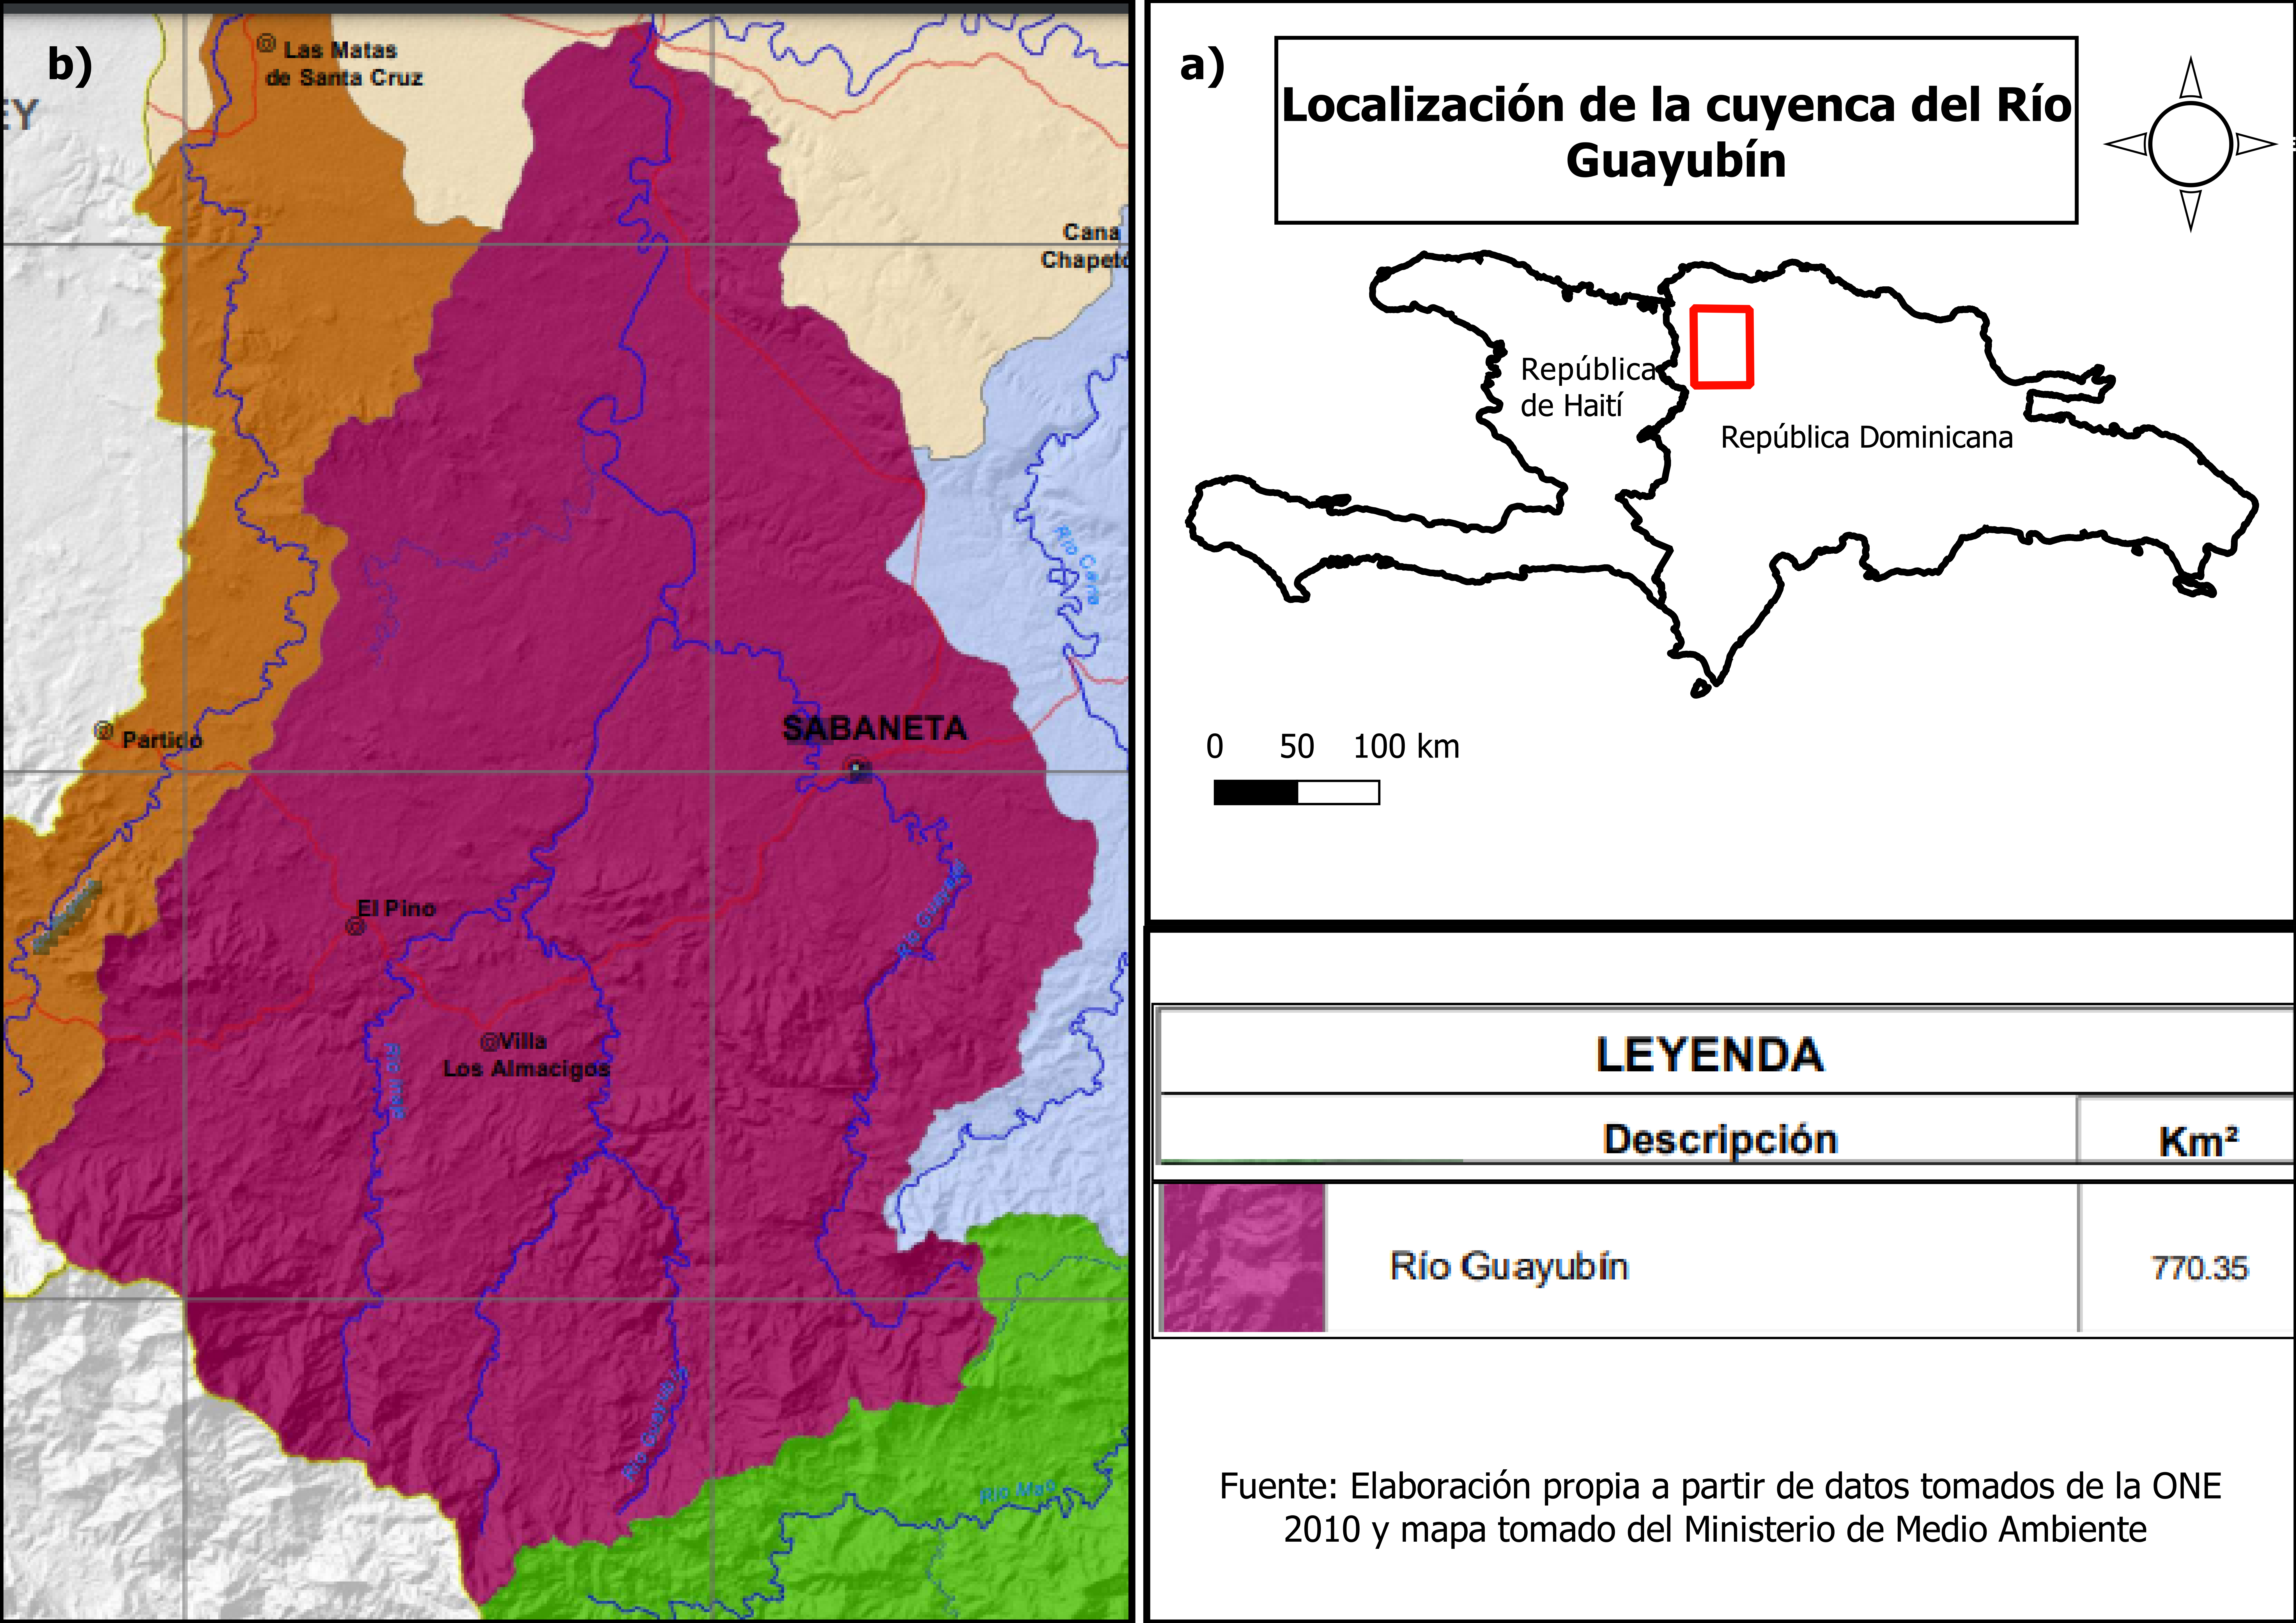
\includegraphics[width=1.00000\textwidth]{Mapa final.png}
\caption{Cuenca del río Guayubín\label{mapacuenca}}
\end{figure}

\section{Materiales y Metodología}\label{materiales-y-metodologuxeda}

Para el estudio morfométrico de la cuenca Guayubín se usó softwares de
código abierto como medio para procesar datos estadísticos y modelos
digitales con la finalidad de generar las informaciones ha analizar e
interpretar.

\subsection{Materiales}\label{materiales}

\begin{longtable}[]{@{}cc@{}}
\toprule
\begin{minipage}[b]{0.11\columnwidth}\centering\strut
Materiales\strut
\end{minipage} & \begin{minipage}[b]{0.83\columnwidth}\centering\strut
Uso\strut
\end{minipage}\tabularnewline
\midrule
\endhead
\begin{minipage}[t]{0.11\columnwidth}\centering\strut
RStudio\strut
\end{minipage} & \begin{minipage}[t]{0.83\columnwidth}\centering\strut
donde se redactó el manuscrito, se procesaron los datos que ofrece el
DEM de la cuenca a traves de un script en el que se usaron paquetes que
produjeran los resultados.\strut
\end{minipage}\tabularnewline
\begin{minipage}[t]{0.11\columnwidth}\centering\strut
library rgrass7\strut
\end{minipage} & \begin{minipage}[t]{0.83\columnwidth}\centering\strut
es una interfaz que permite establecer una conexión entre la version 7
del sistema de infromacion geográfica GRASS, y R, que crea un entorno
GRASS desechable dentro de R.\strut
\end{minipage}\tabularnewline
\begin{minipage}[t]{0.11\columnwidth}\centering\strut
library sp\strut
\end{minipage} & \begin{minipage}[t]{0.83\columnwidth}\centering\strut
este paquete sirve para la importación, manipulación y exportación de
datos espaciales en R, y para métodos que incluyen imprimir / mostrar,
trazar, entre otros.\strut
\end{minipage}\tabularnewline
\begin{minipage}[t]{0.11\columnwidth}\centering\strut
library sf\strut
\end{minipage} & \begin{minipage}[t]{0.83\columnwidth}\centering\strut
crea caracteristicas simples (simple features), que amplían los objetos
tipo data.frame con una columna de lista de características
simples.\strut
\end{minipage}\tabularnewline
\begin{minipage}[t]{0.11\columnwidth}\centering\strut
library raster\strut
\end{minipage} & \begin{minipage}[t]{0.83\columnwidth}\centering\strut
este paquete proporciona clases y funciones para manipular datos
geográficos (espaciales) en formato `ráster'.\strut
\end{minipage}\tabularnewline
\begin{minipage}[t]{0.11\columnwidth}\centering\strut
library leaflet\strut
\end{minipage} & \begin{minipage}[t]{0.83\columnwidth}\centering\strut
esta función crea un widget de mapa de folletos utilizando htmlwidgets.
El widget se puede representar en páginas HTML generadas a partir de R
Markdown, y otros.\strut
\end{minipage}\tabularnewline
\begin{minipage}[t]{0.11\columnwidth}\centering\strut
library leafem\strut
\end{minipage} & \begin{minipage}[t]{0.83\columnwidth}\centering\strut
es un paquete que provee una extensión para leaflet uasados para
paquetes mapview, permite mostrar las coordenadas de la posición del
puntero del mouse, consultar valores de imagen a través de puntero del
mouse y botones de zoom a capa.\strut
\end{minipage}\tabularnewline
\begin{minipage}[t]{0.11\columnwidth}\centering\strut
library mapview\strut
\end{minipage} & \begin{minipage}[t]{0.83\columnwidth}\centering\strut
el paquete proporciona funcionalidad para ver objetos espaciales de
forma interactiva.\strut
\end{minipage}\tabularnewline
\begin{minipage}[t]{0.11\columnwidth}\centering\strut
library readr\strut
\end{minipage} & \begin{minipage}[t]{0.83\columnwidth}\centering\strut
el objetivo de `readr' es proporcionar una forma rápida y amigable de
leer datos rectangulares (como `csv', `tsv' y `fwf').\strut
\end{minipage}\tabularnewline
\begin{minipage}[t]{0.11\columnwidth}\centering\strut
QGIS with GRASS\strut
\end{minipage} & \begin{minipage}[t]{0.83\columnwidth}\centering\strut
para la visualización de vectores y rasters generados con RStudio en una
región de GRASS,como la visualización de los mapas Topológicos y
Geológicos de la República Dominicana, tambien, para la creación de
algunos mapas de localización.\strut
\end{minipage}\tabularnewline
\begin{minipage}[t]{0.11\columnwidth}\centering\strut
Google Earth\strut
\end{minipage} & \begin{minipage}[t]{0.83\columnwidth}\centering\strut
para observar datos en formato kml generados y exportados de RStudio y
asi como la representacion del relieve del lugar de estudio.\strut
\end{minipage}\tabularnewline
\begin{minipage}[t]{0.11\columnwidth}\centering\strut
Mapa Topológico de RD\strut
\end{minipage} & \begin{minipage}[t]{0.83\columnwidth}\centering\strut
para hacer comparaciones y obtener referencias sobre el relieve.\strut
\end{minipage}\tabularnewline
\begin{minipage}[t]{0.11\columnwidth}\centering\strut
Mapa Geológico Nacional de RD\strut
\end{minipage} & \begin{minipage}[t]{0.83\columnwidth}\centering\strut
para hacer comparaciones y obtener referencias sobre la composición
rocosa y los años que datan estas.\strut
\end{minipage}\tabularnewline
\bottomrule
\end{longtable}

\subsection{Metodología}\label{metodologuxeda}

Para el desarrolo del estudio lo primero a realizar fue crear una region
de GRASS en R, importar fuentes y definir la extensión y resolución
(DEM). Luego, explorar básicos entre GRASS y R.

\subsubsection{Aspecto de la cuenca y de la red de
drenaje.}\label{aspecto-de-la-cuenca-y-de-la-red-de-drenaje.}

Los parametros de la cuenca fueron calculados por medio de el addon de
GRASS GIS \texttt{r.watershed} (Charles Ehlschlaeger (2003--2021b)),
utilizando un Dem. Los parametros calculados fueron acumulación,
elevación, depresión, drenaje, flujo, cuenca y media cuenca, con un
umbral de acumulación de flujo de 80 celdas necesarias para que exista
una red de agua. Luego, las capas generadas fueron ingresadas a R con la
\texttt{librería\ sp} y manejadas con la \texttt{librería\ raster}. Se
usó el addon \texttt{r.water.outlet} (Charles Ehlschlaeger
(2003--2021a)) para la extraccion de la cuenca se usaron los parametros
siguientes: de entrada un mapa de direccion de drenajes (creado con el
addon \texttt{r.watershed}), de coordenadas de desembocadura de la
cuenca (obtenidas con la \texttt{librería\ Mapview}), y de salida el
nombre de la cuenca. Asi mismo, se usó el addon \texttt{r.to.vect} (Team
(2003--2021)), para convertir el raster resultante en vectorial, con los
parametros a continuación: de entrada el mapa raster de la cuenca, de
salida el nombre del vectorial y para la característica de salida se usó
el área. Al final de la operación los resultados fueron llevados a R.
Para estraer la red de drenaje se aplico el addon
\texttt{r.stream.extract} (Metz (2003--2021)), usando los parametros:
elevación, umbral de acumulación, mapa raster de flujos y mapa vectorial
de flujos. Luego los resultados de este procedimiento fueron llevados a
R.

\subsubsection{Orden de red y análisis
hortoniano.}\label{orden-de-red-y-anuxe1lisis-hortoniano.}

En cuanto al orden de red y el análisis hortoniano, se usó el addon
\texttt{r.stream.extract} (Metz (2003--2021)), para producir un mapa de
dirección de flujo con los parametros: de entrada un modelo de
elevación, un umbral de acumulación y de sálida el nombre del mapa. Para
la creación de mapas de ordenes de redes generados con
\texttt{r.stream.order} (Jasiewicz (2003--2021)) se usaron los
parametros: de entrada un mapa raster de red de arroyos, un modelo de
elevación, un mapa de direccion de flujos, un mapa de acumulación, de
sálida un vector con todos los atributos de los fliujos, y a sálida de
los vectores con los ordenes de redes según Strahler, Horton, Shreve,
Hack y Topo. Para analizar el orden de red de la cuenca se utilizó la
clasificación de Strahler. Mientras que se usaron los addons
\texttt{r.info} (Michael O'Shea (2003--2021)), para obtener los valores
minimos y maximos del orden de red segun Strahler a partir de un raster;
para delimitar la cuenca a traves de la red de drenaje se utilizo
\texttt{r.stream.basins} (Jarek Jasiewicz \& Institute (2003--2021a)),
los parametros usados son: de entrada un mapa de direccion de flujos, un
mapa mascara de flujos, rango de valores de categorias, y de sálida el
nombre del mapa. En cuanto a las estadísticas según orden de red de
Horton para las redes de Strahler y Horton se uso el addon
\texttt{r.stream.stats} (Jarek Jasiewicz \& Institute (2003--2021b)),
para resumir las estadisticas; los parámetros a usados fueron: de
entrada un raster de red de arroyos, un raster de dirección de flujos,
un modelo de elevación y de sálida el nombre del archivo.

\subsubsection{Índices de concavidad y perfiles
longitudinales.}\label{uxedndices-de-concavidad-y-perfiles-longitudinales.}

Para calcular los índices de concavidad y los perfiles longitudinales,
primero, se obtuvieron los cursos mas largos de la cuenca a traves de la
función \texttt{LfpNetwork} (Batlle (2018b)), usando coordenadas de
desembocadura de la cuenca obtenidas con la \texttt{librería\ Mapview},
vectores de ordenes de red, mapa de flujo de dirección y un sufijo de
sálida para los resultados que se generen. Segundo, para producir los
perfiles longitudinales e índices de cocavidad se empleo la función
\texttt{LfpProfilesConcavity} (Batlle (2018c)), utilizando como
parámetro la red de cursos de agua más largos, coordenadas de
desembocadura, un dem, un mapa de flujos de drenaje, un prefijo, un
sistema de referencia de coordenadas, un parametro de suavizado y un
número de filas de los perfiles.

\subsubsection{Morfometría de cuenca.}\label{morfometruxeda-de-cuenca.}

Tras crear una nueva región de GRASS en R, se continuó con convertir a
números enteros la extensión y la resolución del DEM con las funciones
\texttt{integerextent} (Batlle (2020a)), y \texttt{xyvector} (Batlle
(2018d)). Tambien, se usó la herramienta \texttt{gdalwarp} (Frank
Warmerdam \& others (1998--2021)), para reproyectar y deformar raster.
Se utilizaron los addons \texttt{g.proj} (Kelly (2003--2021)), y
\texttt{r.in.gdal} (Warmerdam (2003--2021)), para importar a la sesion
de GRASS. Se usó el addon \texttt{r.stream.extract} (Metz (2003--2021)),
para generar una red de drenaje y obtener coordenadas a continuación, y
que serían, luego, transformadas a EPSG (MappingGis (2016)), como número
entero con la función \texttt{My\_Trans} (Batlle (2020b)). En cuanto a
la obtención de los parámetros morfométricos de la cuenca se usa el
addon \texttt{r.basin} (Margherita Di Leo (2003--2021)), con los
parámetros siguientes: un modelo de elevación, un prefijo de sálida,
coordenadas de la sálida de la cuenca, umbral de acumulación, y un
directorio donde se ubicará el archivo de salida. Los vectores obtenidos
cson transformados a EPGS (MappingGis (2016)), y asi visualizar con la
\texttt{librería\ Leaflet}. Y para poder explorar los parámetros de la
cuenca se usó la \texttt{librería\ Readr}. Finalmente, para el cálculo
de la curva y la integral hipsométrica, lo primero fue representar las
cuencas con las librerías \texttt{Sp} \texttt{Mapview}; y segundo,
calcular la integral y curva hipsométrica utilizando la función
\texttt{HypsoIntCurve} (Batlle (2018a)), usando de parámetros los
vectores de arroyos de cuenca de orden 2 y 3, un modelo de elevación, un
asignador de campos, el número de filas y una etiqueta de tamaño.

\section{Resultados}\label{resultados}

El fruto del estudio realizado a la cuenca del río Guayubín aplicando la
metodología anterior, produce información que facilita el análisis y
comprensión de la cuenca fluvial, tanto de manera agrupada, como de
forma desagregada.

\subsection{Aspecto general de la cuenca y de la red de
drenaje.}\label{aspecto-general-de-la-cuenca-y-de-la-red-de-drenaje.}

Tras cálcular los parámetros hidrograficos de la cuenca con
\texttt{r.watershed} se obtuvo un raster de tres grupos de capas (DEM,
basins y str), que con la ayuda de \texttt{leaflet} se visualiza un mapa
mostrando las subcuencas, las redes fluviales y el DEM, de la cuenca sin
delimitar. (Ver figura\ref{capas}).

\begin{figure}
\centering
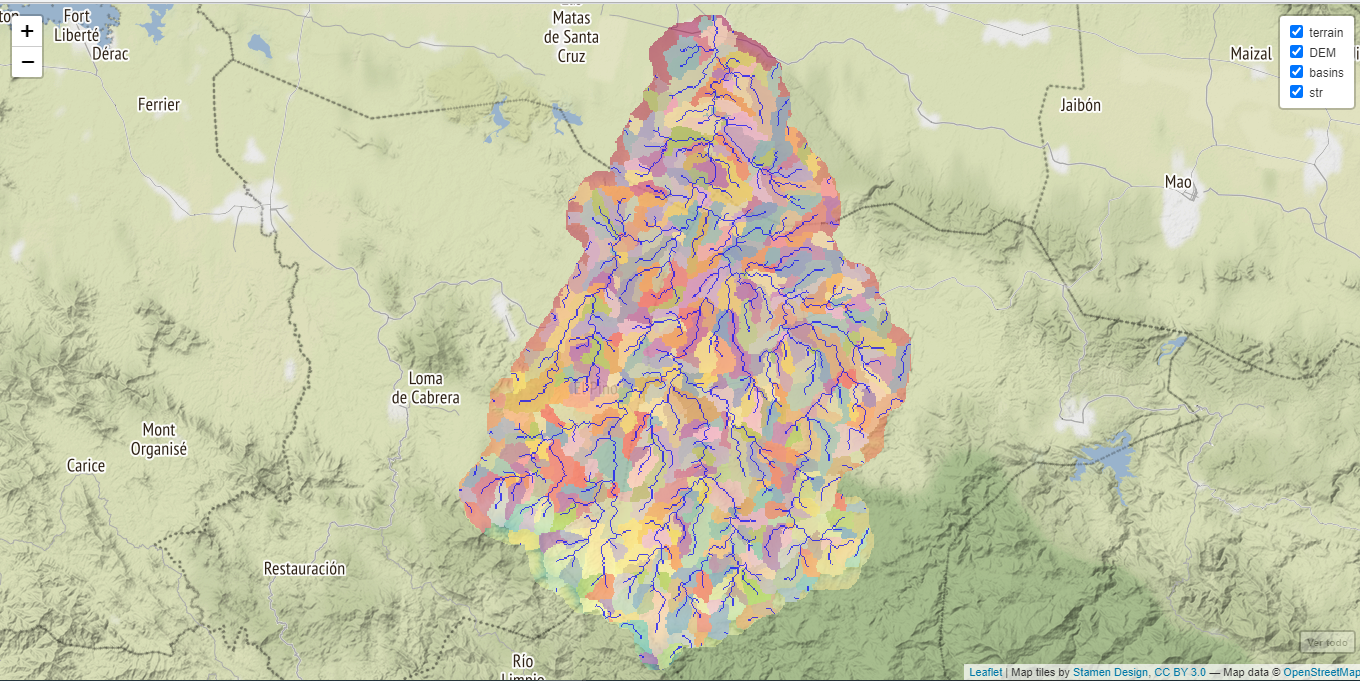
\includegraphics[width=0.60000\textwidth]{capas.png}
\caption{Capas generadas al calcular los parámetros hidrográficos de la
cuenca\label{capas}}
\end{figure}

La cuenca extraida con \texttt{r.water.outlet} produjo un raster de
cuenca delimitada denominado \texttt{guayubin-basin}, que luego paso a
ser un vector llamado \texttt{guayubin\_basin} usando el addon
\texttt{r.to.vect}. (Ver figura\ref{cuencavectorial}). Tras ser llevada
la cuenca ser llevada a R como vector, obtuvo el nombre
\texttt{guayu\_bas}. Aqui representada con \texttt{leaflet} (ver
figura\ref{cuenca delimitada})

\begin{figure}
\centering
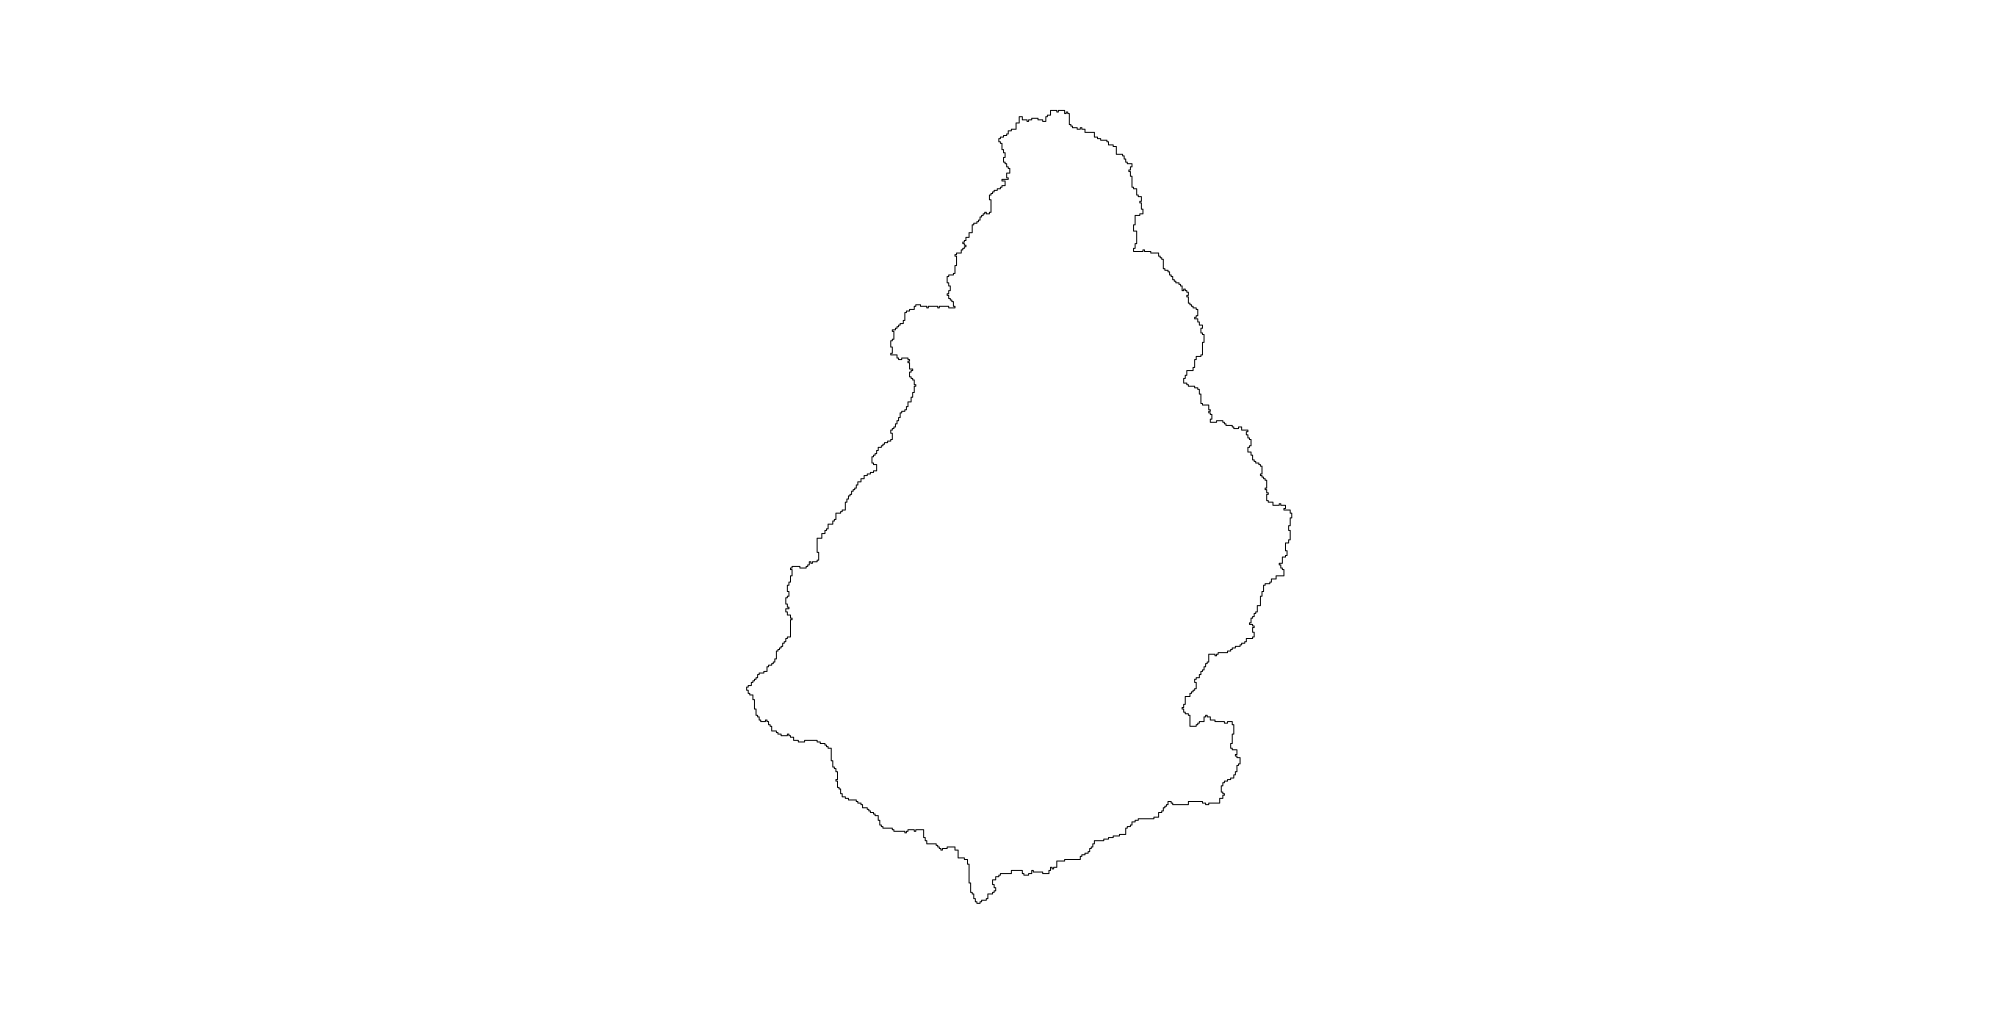
\includegraphics[width=0.50000\textwidth]{cuenca extraida.png}
\caption{Vectorial de la cuenca del río Guayubín\label{cuencavectorial}}
\end{figure}

\begin{figure}
\centering
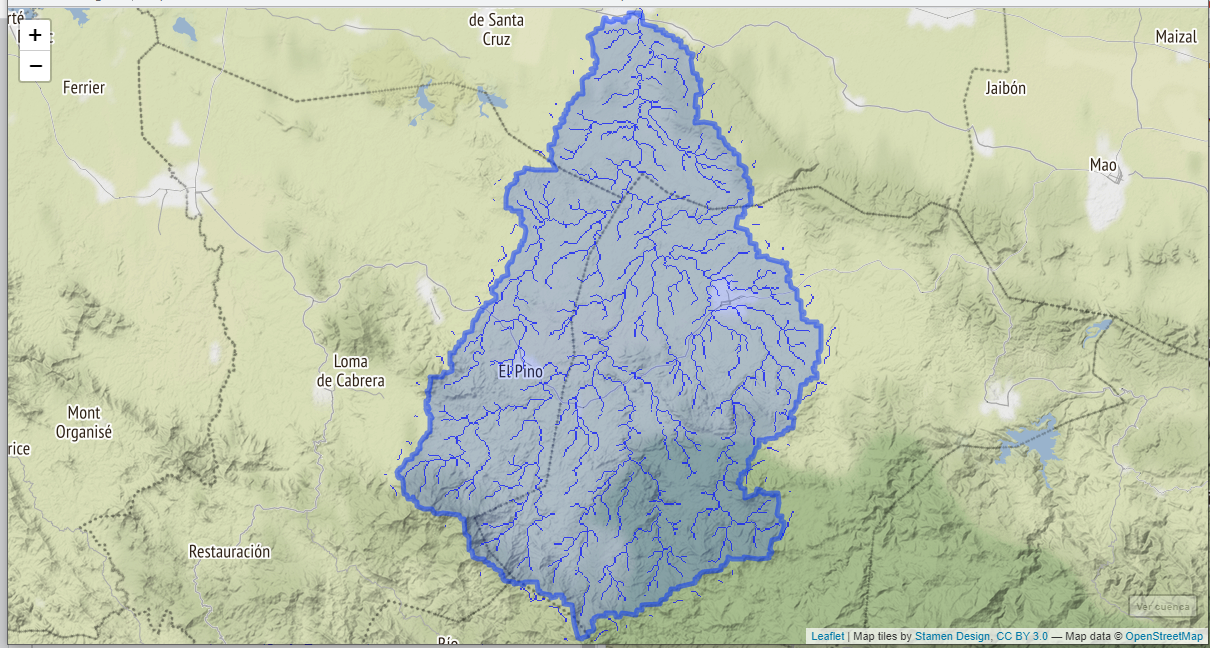
\includegraphics[width=0.50000\textwidth]{cuenca delimitada.png}
\caption{Cuenca del río Guayubín delimitada\label{cuenca delimitada}}
\end{figure}

En cuanto a la red de drenaje extraida con \texttt{r.stream.extract} se
generó un raster y un vector con redes fluviales formadas a partir de un
umbral de 80 celdas, denominados \texttt{guayubin-stream-de-rstr} y
\texttt{guayubin\_stream\_de\_rstr}, respectivamente. Estos productos
tras ser llevados a R, como \texttt{guayu\_net} para el vector y
\texttt{guayu\_net\_r} para el raster. Estos pueden ser visualizados con
\texttt{leaflet} (ver figura\ref{red de drenaje extraida}).

\begin{figure}
\centering
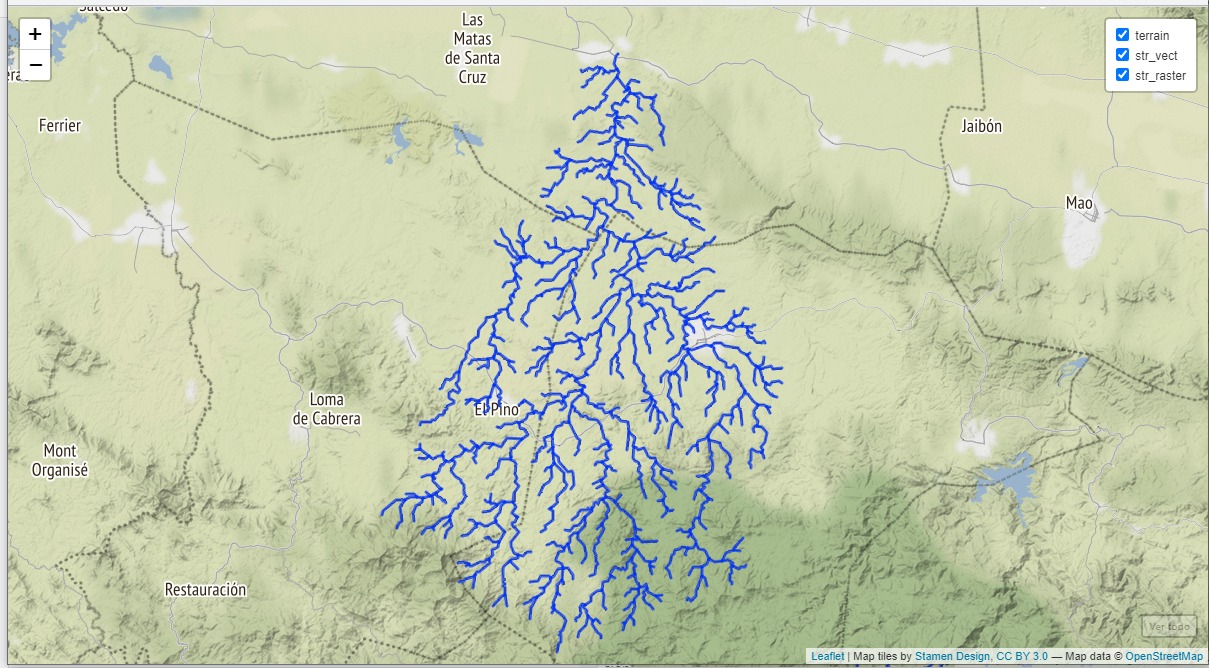
\includegraphics[width=0.70000\textwidth]{red de drenaje extraida.png}
\caption{Red de drenaje del río Guayubín\label{red de drenaje extraida}}
\end{figure}

\subsection{Orden de red analisis
hortoniano}\label{orden-de-red-analisis-hortoniano}

Con el addon \texttt{r.stream.extract} se creó un mapa raster de
direccion de flujos de nombre \texttt{drainage-dir-de-rstr}. Mientras
que con el addons \texttt{r.stream.order} se generaró un vector que
contiene los atributos de la red (\texttt{order\_all}), y mapas rasters
de ordenes de red basados en las clasificaciones de Strahler, Horton,
Shreve, Hack y Topo (Jasiewicz (2003--2021)). Aqui visualizada la capa
vectorial de todos los ordenes con simbologia unica, en \texttt{leaflet}
(ver figura\ref{unica}). Aqui visualizada en \texttt{leaflet} con
simbologia que aplica grosor segun su orden de red (ver
figura\ref{grosor}).

\begin{figure}
\centering
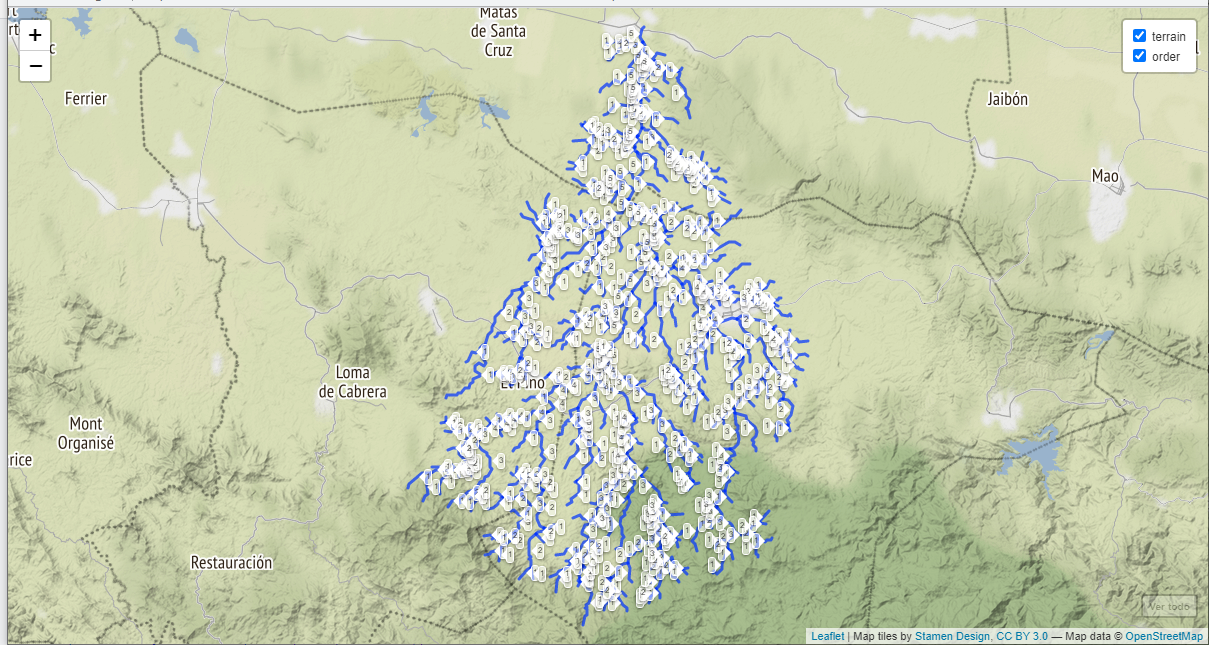
\includegraphics[width=0.50000\textwidth]{ordenes de red.png}
\caption{Ordenes de red del rio Guayubin con simbologia
unica\label{unica}}
\end{figure}

\begin{figure}
\centering
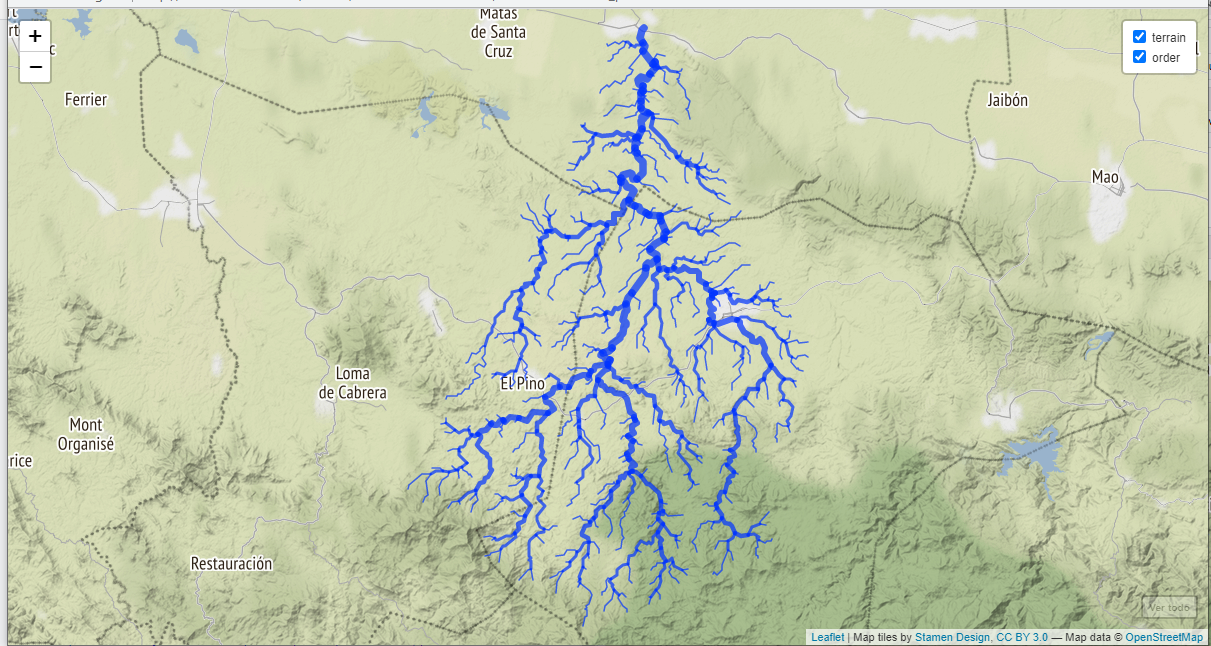
\includegraphics[width=0.50000\textwidth]{orden de red mapa 2.png}
\caption{Ordenes de red del rio Guayubin con simbologia aplicando grosor
segun su orden\label{grosor}}
\end{figure}

Se ordenó y clasificó cada tramo fluvial de la cuenca según Strahler
donde usando el addon \texttt{r.info}, se obtuvo el orden de red máximo
es 5 y el minimo es de 1 . Despues de delimitar las cuencas con
\texttt{r.basin}, se genero un raster que se transformo a vectorial.
Aqui se visualizan las cuencas delimitadas y los ordenes de red (ver
figura\ref{subcuencas}).

\begin{figure}
\centering
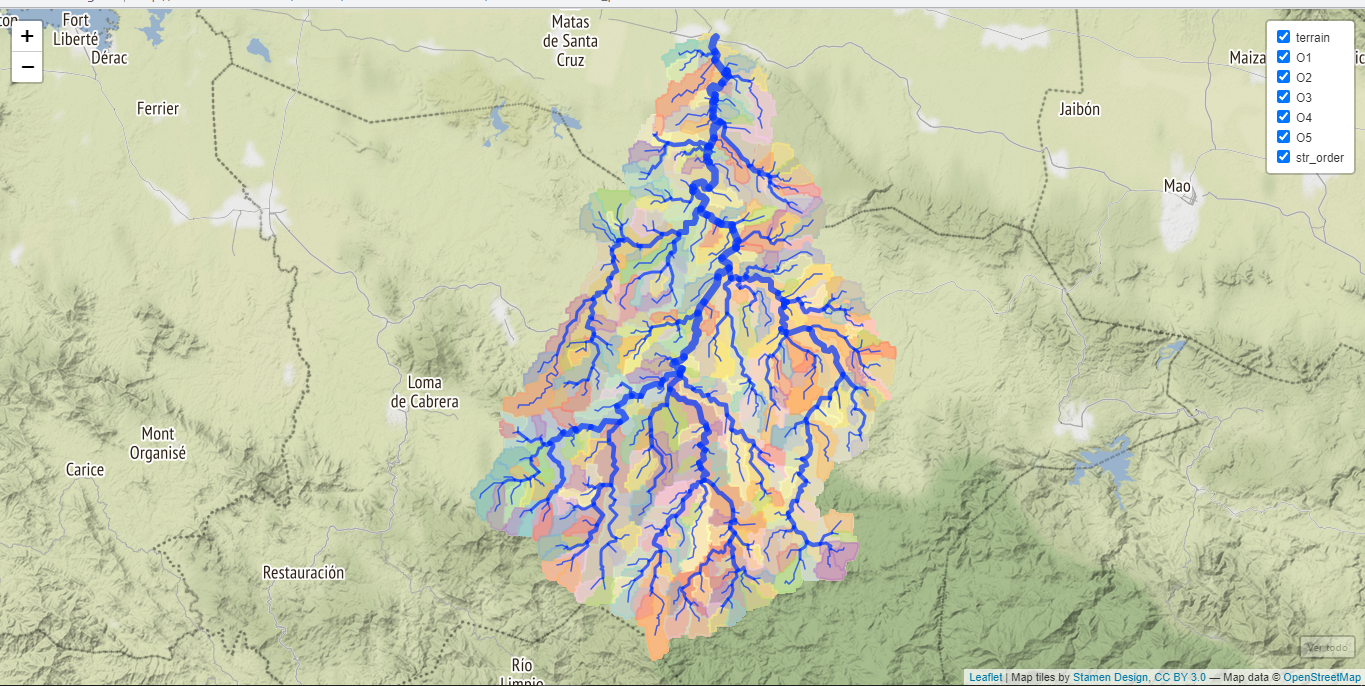
\includegraphics[width=0.70000\textwidth]{cuencas delimitadas y ordenes de red.png}
\caption{Subcuencas y ordenes de red del rio Guayubin\label{subcuencas}}
\end{figure}

Las estadísticas de red resumidas por orden de red según la
clasificación de Strahler, obtenidas con \texttt{r.stream.stats}, se
produjo un documento resumido de sobre los ordenes de red, con esto
mismo fue posible calcular la razon de bifurcacion (4.064346). (ver
figura\ref {grafnumero}).

\begin{figure}
\centering
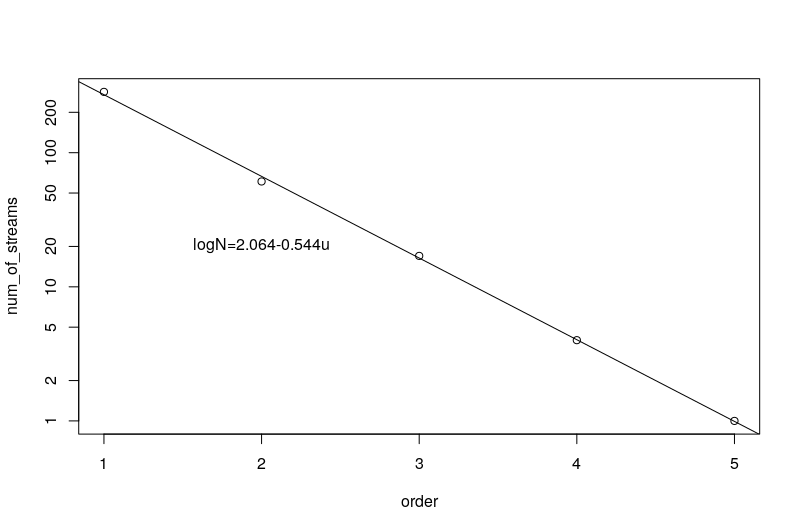
\includegraphics[width=0.80000\textwidth]{Numero de red segun su orden.png}
\caption{Número de redes segun su orden y Razon de bifurcacion por medio
de coeficientes de regresion\label{grafnumero}}
\end{figure}

Asi tambien se obtuvieron con el mismo addon \texttt{r.stream.stats},
estadisticas mas amplias sobre la red.

Summary:

\begin{longtable}[]{@{}cccccc@{}}
\toprule
Max order & Tot.N.str. & Tot.str.len. & Tot.area. & Dr.dens. &
Str.freq.\tabularnewline
\midrule
\endhead
(num) & (num) & (km) & (km\textsuperscript{2}) &
(km/km\textsuperscript{2}) & (num/km\textsuperscript{2})\tabularnewline
5 & 367 & 693.6069 & 773.2235 & 0.8970 & 0.4746\tabularnewline
\bottomrule
\end{longtable}

Stream ratios based on regression coefficient:

\begin{longtable}[]{@{}ccccc@{}}
\toprule
Bif.rt. & Len.rt. & Area.rt. & Slo.rt. & Grd.rt.\tabularnewline
\midrule
\endhead
4.0643 & 2.2928 & 4.5845 & 1.4798 & 1.8338\tabularnewline
\bottomrule
\end{longtable}

Averaged stream ratios with standard deviations:

\begin{longtable}[]{@{}ccccc@{}}
\toprule
Bif.rt. & Len.rt. & Area.rt. & Slo.rt. & Grd.rt.\tabularnewline
\midrule
\endhead
4.1235 & 2.3822 & 3.3126 & 1.4938 & 1.9010\tabularnewline
0.4476 & 0.6025 & 2.2153 & 0.0960 & 0.5050\tabularnewline
\bottomrule
\end{longtable}

\begin{longtable}[]{@{}cccccc@{}}
\toprule
\begin{minipage}[b]{0.08\columnwidth}\centering\strut
Order num\strut
\end{minipage} & \begin{minipage}[b]{0.11\columnwidth}\centering\strut
Avg.len (km)\strut
\end{minipage} & \begin{minipage}[b]{0.25\columnwidth}\centering\strut
Avg.ar (km\textsuperscript{2})\strut
\end{minipage} & \begin{minipage}[b]{0.11\columnwidth}\centering\strut
Avg.sl (m/m)\strut
\end{minipage} & \begin{minipage}[b]{0.14\columnwidth}\centering\strut
Avg.grad. (m/m)\strut
\end{minipage} & \begin{minipage}[b]{0.13\columnwidth}\centering\strut
Avg.el.dif (m)\strut
\end{minipage}\tabularnewline
\midrule
\endhead
\begin{minipage}[t]{0.08\columnwidth}\centering\strut
1\strut
\end{minipage} & \begin{minipage}[t]{0.11\columnwidth}\centering\strut
1.2435\strut
\end{minipage} & \begin{minipage}[t]{0.25\columnwidth}\centering\strut
1.7188\strut
\end{minipage} & \begin{minipage}[t]{0.11\columnwidth}\centering\strut
0.0367\strut
\end{minipage} & \begin{minipage}[t]{0.14\columnwidth}\centering\strut
0.0296\strut
\end{minipage} & \begin{minipage}[t]{0.13\columnwidth}\centering\strut
37.4437\strut
\end{minipage}\tabularnewline
\begin{minipage}[t]{0.08\columnwidth}\centering\strut
2\strut
\end{minipage} & \begin{minipage}[t]{0.11\columnwidth}\centering\strut
2.4743\strut
\end{minipage} & \begin{minipage}[t]{0.25\columnwidth}\centering\strut
7.2904\strut
\end{minipage} & \begin{minipage}[t]{0.11\columnwidth}\centering\strut
0.0246\strut
\end{minipage} & \begin{minipage}[t]{0.14\columnwidth}\centering\strut
0.0201\strut
\end{minipage} & \begin{minipage}[t]{0.13\columnwidth}\centering\strut
49.0820\strut
\end{minipage}\tabularnewline
\begin{minipage}[t]{0.08\columnwidth}\centering\strut
3\strut
\end{minipage} & \begin{minipage}[t]{0.11\columnwidth}\centering\strut
6.2881\strut
\end{minipage} & \begin{minipage}[t]{0.25\columnwidth}\centering\strut
31.7328\strut
\end{minipage} & \begin{minipage}[t]{0.11\columnwidth}\centering\strut
0.0165\strut
\end{minipage} & \begin{minipage}[t]{0.14\columnwidth}\centering\strut
0.0113\strut
\end{minipage} & \begin{minipage}[t]{0.13\columnwidth}\centering\strut
85.1765\strut
\end{minipage}\tabularnewline
\begin{minipage}[t]{0.08\columnwidth}\centering\strut
4\strut
\end{minipage} & \begin{minipage}[t]{0.11\columnwidth}\centering\strut
11.5356\strut
\end{minipage} & \begin{minipage}[t]{0.25\columnwidth}\centering\strut
147.7492\strut
\end{minipage} & \begin{minipage}[t]{0.11\columnwidth}\centering\strut
0.0120\strut
\end{minipage} & \begin{minipage}[t]{0.14\columnwidth}\centering\strut
0.0066\strut
\end{minipage} & \begin{minipage}[t]{0.13\columnwidth}\centering\strut
80.0000\strut
\end{minipage}\tabularnewline
\begin{minipage}[t]{0.08\columnwidth}\centering\strut
5\strut
\end{minipage} & \begin{minipage}[t]{0.11\columnwidth}\centering\strut
36.4888\strut
\end{minipage} & \begin{minipage}[t]{0.25\columnwidth}\centering\strut
773.2235\strut
\end{minipage} & \begin{minipage}[t]{0.11\columnwidth}\centering\strut
0.0074\strut
\end{minipage} & \begin{minipage}[t]{0.14\columnwidth}\centering\strut
0.0025\strut
\end{minipage} & \begin{minipage}[t]{0.13\columnwidth}\centering\strut
91.0000\strut
\end{minipage}\tabularnewline
\bottomrule
\end{longtable}

\begin{longtable}[]{@{}cccccc@{}}
\toprule
\begin{minipage}[b]{0.08\columnwidth}\centering\strut
Order num\strut
\end{minipage} & \begin{minipage}[b]{0.11\columnwidth}\centering\strut
Std.len (km)\strut
\end{minipage} & \begin{minipage}[b]{0.26\columnwidth}\centering\strut
Std.ar (km\textsuperscript{2})\strut
\end{minipage} & \begin{minipage}[b]{0.11\columnwidth}\centering\strut
Std.sl (m/m)\strut
\end{minipage} & \begin{minipage}[b]{0.14\columnwidth}\centering\strut
Std.grad. (m/m)\strut
\end{minipage} & \begin{minipage}[b]{0.13\columnwidth}\centering\strut
Std.el.dif (m)\strut
\end{minipage}\tabularnewline
\midrule
\endhead
\begin{minipage}[t]{0.08\columnwidth}\centering\strut
1\strut
\end{minipage} & \begin{minipage}[t]{0.11\columnwidth}\centering\strut
1.0274\strut
\end{minipage} & \begin{minipage}[t]{0.26\columnwidth}\centering\strut
1.0955\strut
\end{minipage} & \begin{minipage}[t]{0.11\columnwidth}\centering\strut
0.0379\strut
\end{minipage} & \begin{minipage}[t]{0.14\columnwidth}\centering\strut
0.0324\strut
\end{minipage} & \begin{minipage}[t]{0.13\columnwidth}\centering\strut
52.7742\strut
\end{minipage}\tabularnewline
\begin{minipage}[t]{0.08\columnwidth}\centering\strut
2\strut
\end{minipage} & \begin{minipage}[t]{0.11\columnwidth}\centering\strut
1.9695\strut
\end{minipage} & \begin{minipage}[t]{0.26\columnwidth}\centering\strut
4.4097\strut
\end{minipage} & \begin{minipage}[t]{0.11\columnwidth}\centering\strut
0.0215\strut
\end{minipage} & \begin{minipage}[t]{0.14\columnwidth}\centering\strut
0.0194\strut
\end{minipage} & \begin{minipage}[t]{0.13\columnwidth}\centering\strut
52.5830\strut
\end{minipage}\tabularnewline
\begin{minipage}[t]{0.08\columnwidth}\centering\strut
3\strut
\end{minipage} & \begin{minipage}[t]{0.11\columnwidth}\centering\strut
5.0992\strut
\end{minipage} & \begin{minipage}[t]{0.26\columnwidth}\centering\strut
19.0637\strut
\end{minipage} & \begin{minipage}[t]{0.11\columnwidth}\centering\strut
0.0092\strut
\end{minipage} & \begin{minipage}[t]{0.14\columnwidth}\centering\strut
0.0077\strut
\end{minipage} & \begin{minipage}[t]{0.13\columnwidth}\centering\strut
93.4085\strut
\end{minipage}\tabularnewline
\begin{minipage}[t]{0.08\columnwidth}\centering\strut
4\strut
\end{minipage} & \begin{minipage}[t]{0.11\columnwidth}\centering\strut
5.8247\strut
\end{minipage} & \begin{minipage}[t]{0.26\columnwidth}\centering\strut
44.3177\strut
\end{minipage} & \begin{minipage}[t]{0.11\columnwidth}\centering\strut
0.0041\strut
\end{minipage} & \begin{minipage}[t]{0.14\columnwidth}\centering\strut
0.0032\strut
\end{minipage} & \begin{minipage}[t]{0.13\columnwidth}\centering\strut
57.0789\strut
\end{minipage}\tabularnewline
\begin{minipage}[t]{0.08\columnwidth}\centering\strut
5\strut
\end{minipage} & \begin{minipage}[t]{0.11\columnwidth}\centering\strut
-0.0000\strut
\end{minipage} & \begin{minipage}[t]{0.26\columnwidth}\centering\strut
0.0000\strut
\end{minipage} & \begin{minipage}[t]{0.11\columnwidth}\centering\strut
0.0000\strut
\end{minipage} & \begin{minipage}[t]{0.14\columnwidth}\centering\strut
0.0000\strut
\end{minipage} & \begin{minipage}[t]{0.13\columnwidth}\centering\strut
0.0000\strut
\end{minipage}\tabularnewline
\bottomrule
\end{longtable}

\begin{longtable}[]{@{}cccc@{}}
\toprule
Order & N.streams & Tot.len (km) & Tot.area
(km\textsuperscript{2})\tabularnewline
\midrule
\endhead
1 & 284 & 353.1463 & 488.1383\tabularnewline
2 & 61 & 150.9325 & 444.7173\tabularnewline
3 & 17 & 106.8969 & 539.4576\tabularnewline
4 & 4 & 46.1425 & 590.9969\tabularnewline
5 & 1 & 36.4888 & 773.2235\tabularnewline
\bottomrule
\end{longtable}

\begin{longtable}[]{@{}cccccccc@{}}
\toprule
Order & Bif.rt. & Len.rt. & Area.rt. & Slo.rt. & Grd.rt. & d.dens. &
str.freq.\tabularnewline
\midrule
\endhead
1 & 4.6557 & 1.9898 & 0.0000 & 1.4930 & 1.4748 & 0.7235 &
0.5818\tabularnewline
2 & 3.5882 & 2.5413 & 4.2416 & 1.4930 & 1.7757 & 0.3394 &
0.1372\tabularnewline
3 & 4.2500 & 1.8345 & 4.3527 & 1.3771 & 1.7207 & 0.1982 &
0.0315\tabularnewline
4 & 4.0000 & 3.1631 & 4.6560 & 1.6122 & 2.6327 & 0.0781 &
0.0068\tabularnewline
5 & 0.0000 & 0.0000 & 5.2334 & 0.0000 & 0.0000 & 0.0472 &
0.0013\tabularnewline
\bottomrule
\end{longtable}

\subsection{Índices de concavidad y perfiles
longitudinales}\label{uxedndices-de-concavidad-y-perfiles-longitudinales}

Con la función \texttt{LfpNetwork} obtuvieron los cursos mas largos de
la red de drenaje en formato vectorial y raster, con el sufijo de sálida
\texttt{Gyb}. Para representarlo con \texttt{leaflet} se uso el archivo
vectorial resultante de la operación anterior (ver figura\ref{lfpnet}).

\begin{figure}
\centering
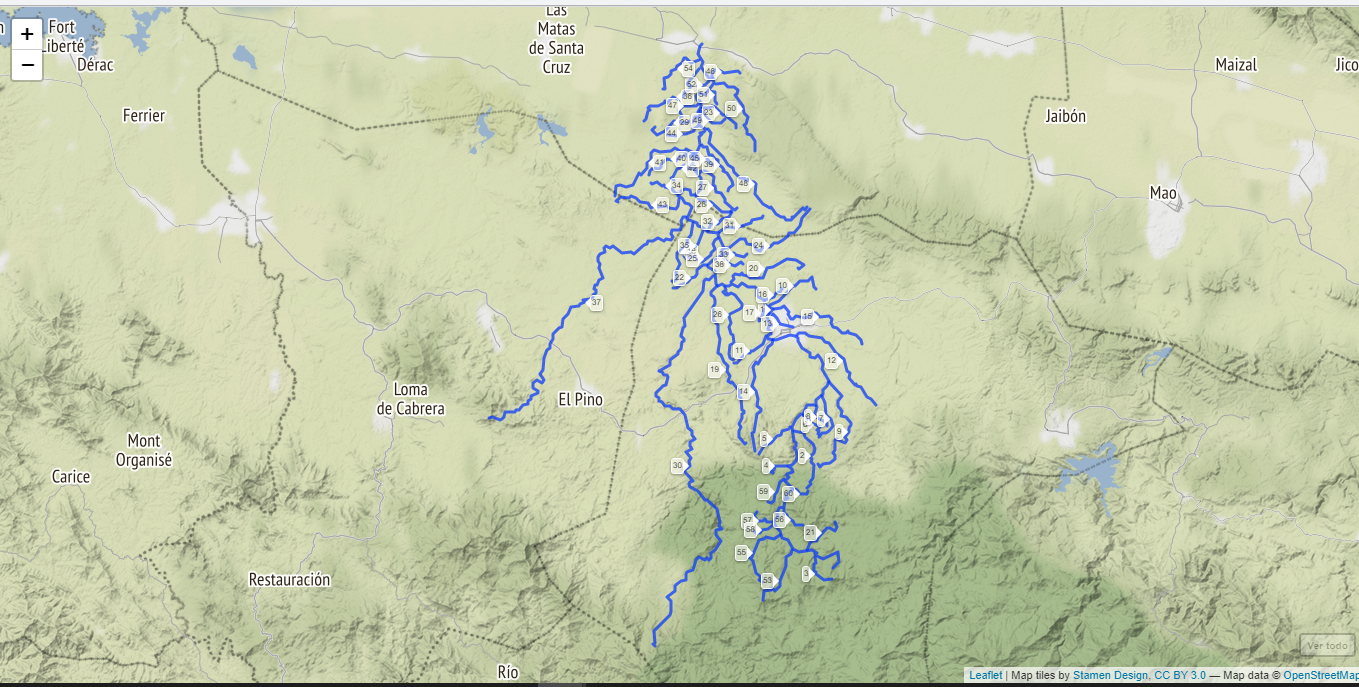
\includegraphics[width=0.60000\textwidth]{cursos mas largos.png}
\caption{Cursos fluviales mas largos de la cuenca del rio
Guayubin\label{lfpnet}}
\end{figure}

Mientras tanto, el producto de aplicar la funcion
\texttt{LfpProfilesConcavity} fueron los perfiles longitudinales (ver
figura\ref{plongitudinal}), y sus indices de concavidad, bajo el prefijo
\texttt{Gyb} (ver figura\ref{indicec}).

\begin{longtable}[]{@{}ccc@{}}
\toprule
stream & stream & ci\tabularnewline
\midrule
\endhead
1 & Gyb-1 & 0.59688059\tabularnewline
2 & Gyb-2 & 0.03127299\tabularnewline
3 & Gyb-3 & 0.29980801\tabularnewline
4 & Gyb-4 & 0.29916212\tabularnewline
5 & Gyb-5 & 0.17766577\tabularnewline
6 & Gyb-6 & 0.28394390\tabularnewline
7 & Gyb-7 & 0.19284167\tabularnewline
8 & Gyb-8 & -0.10206344\tabularnewline
9 & Gyb-9 & 0.08282423\tabularnewline
10 & Gyb-10 & 0.20654655\tabularnewline
11 & Gyb-11 & 0.18245774\tabularnewline
12 & Gyb-12 & 0.41931839\tabularnewline
13 & Gyb-13 & -0.25074216\tabularnewline
14 & Gyb-14 & 0.38778387\tabularnewline
15 & Gyb-15 & 0.09593430\tabularnewline
16 & Gyb-16 & -0.00514126\tabularnewline
17 & Gyb-17 & 0.38870710\tabularnewline
18 & Gyb-18 & -0.12838671\tabularnewline
19 & Gyb-19 & 0.45559497\tabularnewline
20 & Gyb-20 & 0.30800052\tabularnewline
21 & Gyb-21 & 0.31322918\tabularnewline
22 & Gyb-22 & -0.10635769\tabularnewline
23 & Gyb-23 & 0.01957733\tabularnewline
24 & Gyb-24 & 0.44752299\tabularnewline
25 & Gyb-25 & 0.17774471\tabularnewline
26 & Gyb-26 & 0.42982725\tabularnewline
27 & Gyb-27 & 0.15705975\tabularnewline
28 & Gyb-28 & 0.18432963\tabularnewline
29 & Gyb-29 & 0.19728723\tabularnewline
30 & Gyb-30 & 0.59437845\tabularnewline
31 & Gyb-31 & 0.21676465\tabularnewline
32 & Gyb-32 & -0.01923832\tabularnewline
33 & Gyb-33 & 0.31131545\tabularnewline
34 & Gyb-34 & 0.10937291\tabularnewline
35 & Gyb-35 & -0.01857437\tabularnewline
36 & Gyb-36 & 0.38463884\tabularnewline
37 & Gyb-37 & 0.56058882\tabularnewline
38 & Gyb-38 & -0.01128950\tabularnewline
39 & Gyb-39 & 0.33855144\tabularnewline
40 & Gyb-40 & 0.16757638\tabularnewline
41 & Gyb-41 & 0.43546641\tabularnewline
42 & Gyb-42 & 0.08664117\tabularnewline
43 & Gyb-43 & 0.50047621\tabularnewline
44 & Gyb-44 & 0.16043136\tabularnewline
45 & Gyb-45 & 0.05523892\tabularnewline
46 & Gyb-46 & 0.43059893\tabularnewline
47 & Gyb-47 & 0.23599474\tabularnewline
48 & Gyb-48 & 0.51288891\tabularnewline
49 & Gyb-49 & 0.62294206\tabularnewline
50 & Gyb-50 & 0.14796424\tabularnewline
51 & Gyb-51 & 0.28259012\tabularnewline
52 & Gyb-52 & 0.50952086\tabularnewline
53 & Gyb-53 & 0.34383993\tabularnewline
54 & Gyb-54 & 0.39314762\tabularnewline
55 & Gyb-55 & 0.54157833\tabularnewline
56 & Gyb-56 & 0.47292848\tabularnewline
57 & Gyb-57 & 0.26080951\tabularnewline
58 & Gyb-58 & 0.03618367\tabularnewline
59 & Gyb-59 & -0.14210268\tabularnewline
60 & Gyb-60 & 0.19188075\tabularnewline
\bottomrule
\end{longtable}

\begin{figure}
\centering
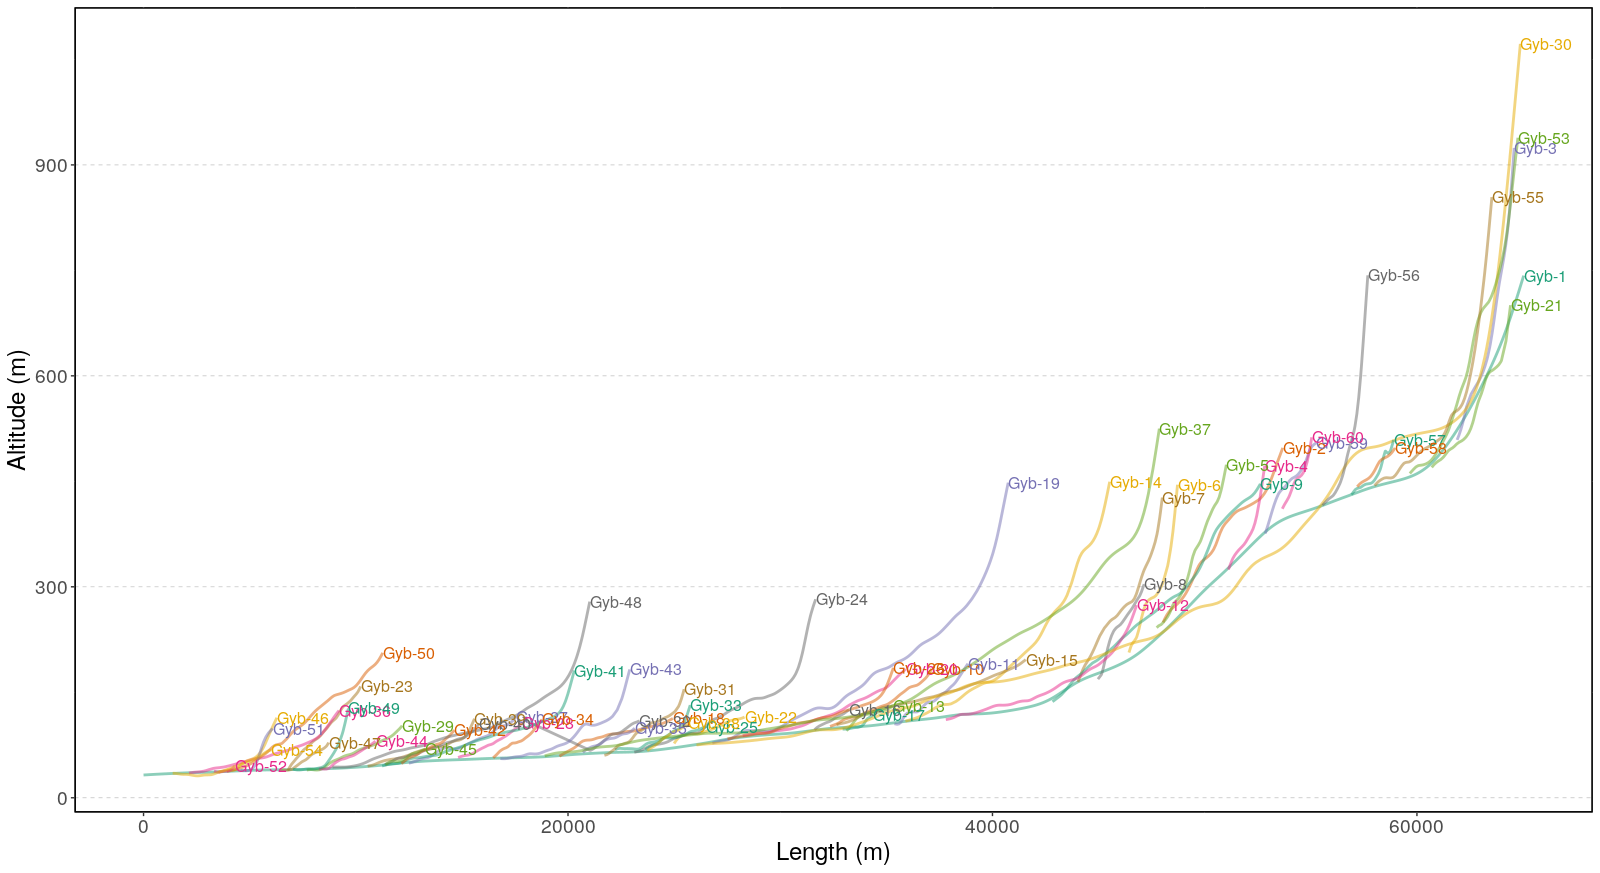
\includegraphics[width=1.00000\textwidth]{perfiles longitudinales.png}
\caption{Perfiles longitudinales de los cursos mas largos en la cuenca
Guayubin\label{plongitudinal}}
\end{figure}

\begin{figure}
\centering
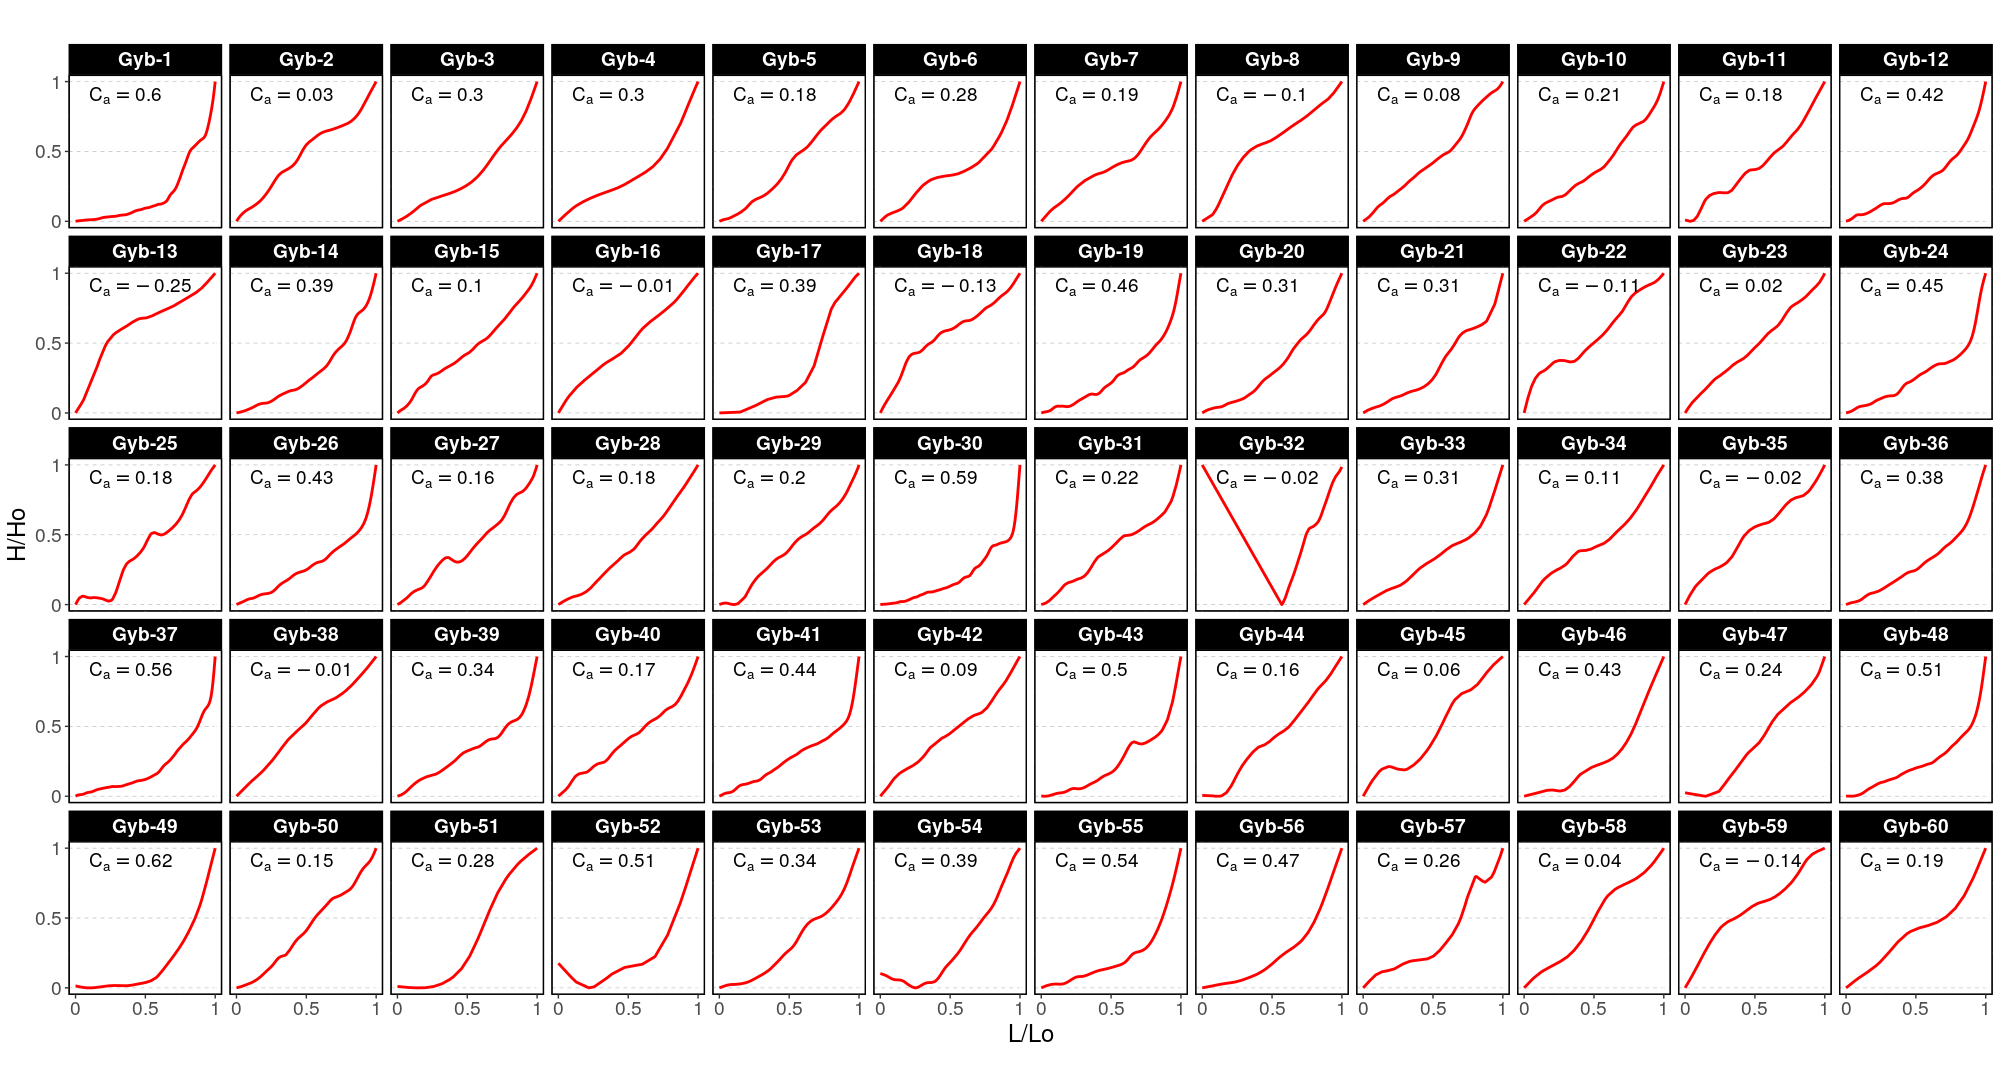
\includegraphics[width=1.00000\textwidth]{Indices de concavidad.png}
\caption{Perfiles longitudinales e indices de concavidad de los cursos
mas largos en la cuenca del rio Guayubin\label{indicec}}
\end{figure}

\subsection{Morfometria de cuenca}\label{morfometria-de-cuenca}

El calculo morfometrico de la cuenca fue realizado con el addon
\texttt{r.basin}, generando vectoriales y raster de la cuenca y de su
red de drenaje. Luego, los vectoriales fueron transformados a
\texttt{EPSG:\ 4326} (ver figura\ref{vectoresrbasin}).

\begin{figure}
\centering
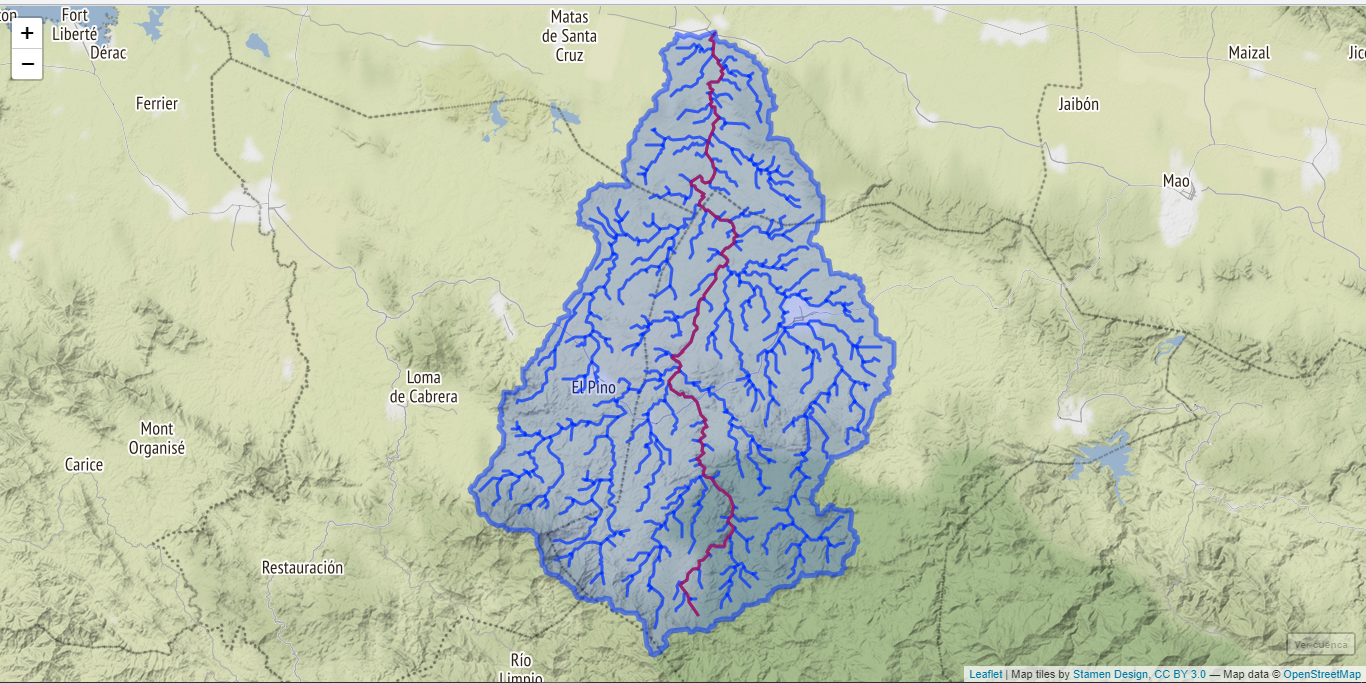
\includegraphics[width=0.50000\textwidth]{cuenca-red de drenaje-curso mas largo.png}
\caption{Cuenca del rio Guayubin con su red de drenaje y su curso mas
largo\label{vectoresrbasin}}
\end{figure}

Parametros morfometricos de la cuenca

\begin{longtable}[]{@{}cc@{}}
\toprule
\begin{minipage}[b]{0.65\columnwidth}\centering\strut
Parametros\strut
\end{minipage} & \begin{minipage}[b]{0.29\columnwidth}\centering\strut
Valores\strut
\end{minipage}\tabularnewline
\midrule
\endhead
\begin{minipage}[t]{0.65\columnwidth}\centering\strut
Easting Centroid of basin\strut
\end{minipage} & \begin{minipage}[t]{0.29\columnwidth}\centering\strut
246465.00\strut
\end{minipage}\tabularnewline
\begin{minipage}[t]{0.65\columnwidth}\centering\strut
Northing Centroid of basin\strut
\end{minipage} & \begin{minipage}[t]{0.29\columnwidth}\centering\strut
2151675.00\strut
\end{minipage}\tabularnewline
\begin{minipage}[t]{0.65\columnwidth}\centering\strut
Rectangle containing basin N-W\strut
\end{minipage} & \begin{minipage}[t]{0.29\columnwidth}\centering\strut
(`230220', `2175930')\strut
\end{minipage}\tabularnewline
\begin{minipage}[t]{0.65\columnwidth}\centering\strut
Rectangle containing basin S-E\strut
\end{minipage} & \begin{minipage}[t]{0.29\columnwidth}\centering\strut
(`261000', `2131290')\strut
\end{minipage}\tabularnewline
\begin{minipage}[t]{0.65\columnwidth}\centering\strut
Area of basin {[}km\^{}2{]}\strut
\end{minipage} & \begin{minipage}[t]{0.29\columnwidth}\centering\strut
773.5631625\strut
\end{minipage}\tabularnewline
\begin{minipage}[t]{0.65\columnwidth}\centering\strut
Perimeter of basin {[}km{]}\strut
\end{minipage} & \begin{minipage}[t]{0.29\columnwidth}\centering\strut
156.122652506552\strut
\end{minipage}\tabularnewline
\begin{minipage}[t]{0.65\columnwidth}\centering\strut
Max Elevation {[}m s.l.m.{]}\strut
\end{minipage} & \begin{minipage}[t]{0.29\columnwidth}\centering\strut
1396.72540740785\strut
\end{minipage}\tabularnewline
\begin{minipage}[t]{0.65\columnwidth}\centering\strut
Min Elevation {[}m s.l.m.{]}\strut
\end{minipage} & \begin{minipage}[t]{0.29\columnwidth}\centering\strut
30.9651954818271\strut
\end{minipage}\tabularnewline
\begin{minipage}[t]{0.65\columnwidth}\centering\strut
Elevation Difference {[}m{]}\strut
\end{minipage} & \begin{minipage}[t]{0.29\columnwidth}\centering\strut
1365.760211926023\strut
\end{minipage}\tabularnewline
\begin{minipage}[t]{0.65\columnwidth}\centering\strut
Mean Elevation\strut
\end{minipage} & \begin{minipage}[t]{0.29\columnwidth}\centering\strut
276.7019\strut
\end{minipage}\tabularnewline
\begin{minipage}[t]{0.65\columnwidth}\centering\strut
Mean Slope\strut
\end{minipage} & \begin{minipage}[t]{0.29\columnwidth}\centering\strut
5.17\strut
\end{minipage}\tabularnewline
\begin{minipage}[t]{0.65\columnwidth}\centering\strut
Length of Directing Vector {[}km{]}\strut
\end{minipage} & \begin{minipage}[t]{0.29\columnwidth}\centering\strut
24.460893544594807\strut
\end{minipage}\tabularnewline
\begin{minipage}[t]{0.65\columnwidth}\centering\strut
Prevalent Orientation {[}degree from north, counterclockwise{]}\strut
\end{minipage} & \begin{minipage}[t]{0.29\columnwidth}\centering\strut
1.4935760627096282\strut
\end{minipage}\tabularnewline
\begin{minipage}[t]{0.65\columnwidth}\centering\strut
Compactness Coefficient\strut
\end{minipage} & \begin{minipage}[t]{0.29\columnwidth}\centering\strut
4.974655054098116\strut
\end{minipage}\tabularnewline
\begin{minipage}[t]{0.65\columnwidth}\centering\strut
Circularity Ratio\strut
\end{minipage} & \begin{minipage}[t]{0.29\columnwidth}\centering\strut
0.3988171279899944\strut
\end{minipage}\tabularnewline
\begin{minipage}[t]{0.65\columnwidth}\centering\strut
Topological Diameter\strut
\end{minipage} & \begin{minipage}[t]{0.29\columnwidth}\centering\strut
84.0\strut
\end{minipage}\tabularnewline
\begin{minipage}[t]{0.65\columnwidth}\centering\strut
Elongation Ratio\strut
\end{minipage} & \begin{minipage}[t]{0.29\columnwidth}\centering\strut
0.5064682945330589\strut
\end{minipage}\tabularnewline
\begin{minipage}[t]{0.65\columnwidth}\centering\strut
Shape Factor\strut
\end{minipage} & \begin{minipage}[t]{0.29\columnwidth}\centering\strut
12.483750895456415\strut
\end{minipage}\tabularnewline
\begin{minipage}[t]{0.65\columnwidth}\centering\strut
Concentration Time (Giandotti, 1934) {[}hr{]}\strut
\end{minipage} & \begin{minipage}[t]{0.29\columnwidth}\centering\strut
6.906840311938352\strut
\end{minipage}\tabularnewline
\begin{minipage}[t]{0.65\columnwidth}\centering\strut
Length of Mainchannel {[}km{]}\strut
\end{minipage} & \begin{minipage}[t]{0.29\columnwidth}\centering\strut
61.965603846\strut
\end{minipage}\tabularnewline
\begin{minipage}[t]{0.65\columnwidth}\centering\strut
Mean slope of mainchannel {[}percent{]}\strut
\end{minipage} & \begin{minipage}[t]{0.29\columnwidth}\centering\strut
1.9669190473941982\strut
\end{minipage}\tabularnewline
\begin{minipage}[t]{0.65\columnwidth}\centering\strut
Mean hillslope length {[}m{]}\strut
\end{minipage} & \begin{minipage}[t]{0.29\columnwidth}\centering\strut
250.4986\strut
\end{minipage}\tabularnewline
\begin{minipage}[t]{0.65\columnwidth}\centering\strut
Magnitudo\strut
\end{minipage} & \begin{minipage}[t]{0.29\columnwidth}\centering\strut
223.0\strut
\end{minipage}\tabularnewline
\begin{minipage}[t]{0.65\columnwidth}\centering\strut
Max order (Strahler)\strut
\end{minipage} & \begin{minipage}[t]{0.29\columnwidth}\centering\strut
5\strut
\end{minipage}\tabularnewline
\begin{minipage}[t]{0.65\columnwidth}\centering\strut
Number of streams\strut
\end{minipage} & \begin{minipage}[t]{0.29\columnwidth}\centering\strut
343\strut
\end{minipage}\tabularnewline
\begin{minipage}[t]{0.65\columnwidth}\centering\strut
Total Stream Length {[}km{]}\strut
\end{minipage} & \begin{minipage}[t]{0.29\columnwidth}\centering\strut
662.2185\strut
\end{minipage}\tabularnewline
\begin{minipage}[t]{0.65\columnwidth}\centering\strut
First order stream frequency\strut
\end{minipage} & \begin{minipage}[t]{0.29\columnwidth}\centering\strut
0.2882763952710843\strut
\end{minipage}\tabularnewline
\begin{minipage}[t]{0.65\columnwidth}\centering\strut
Drainage Density {[}km/km\^{}2{]}\strut
\end{minipage} & \begin{minipage}[t]{0.29\columnwidth}\centering\strut
0.8560626101427108\strut
\end{minipage}\tabularnewline
\begin{minipage}[t]{0.65\columnwidth}\centering\strut
Bifurcation Ratio (Horton)\strut
\end{minipage} & \begin{minipage}[t]{0.29\columnwidth}\centering\strut
3.8876\strut
\end{minipage}\tabularnewline
\begin{minipage}[t]{0.65\columnwidth}\centering\strut
Length Ratio (Horton)\strut
\end{minipage} & \begin{minipage}[t]{0.29\columnwidth}\centering\strut
2.2966\strut
\end{minipage}\tabularnewline
\begin{minipage}[t]{0.65\columnwidth}\centering\strut
Area ratio (Horton)\strut
\end{minipage} & \begin{minipage}[t]{0.29\columnwidth}\centering\strut
4.3704\strut
\end{minipage}\tabularnewline
\begin{minipage}[t]{0.65\columnwidth}\centering\strut
Slope ratio (Horton)\strut
\end{minipage} & \begin{minipage}[t]{0.29\columnwidth}\centering\strut
1.4689\strut
\end{minipage}\tabularnewline
\bottomrule
\end{longtable}

\section{Discusión}\label{discusiuxf3n}

De acuerdo con el s.a. (s.f.), la cabecera del rio Guayubin se ubica en
las inmediaciones de loma escondida

\section{Agradecimientos}\label{agradecimientos}

\section{Información de soporte}\label{informaciuxf3n-de-soporte}

\section{\texorpdfstring{\emph{Script}
reproducible}{Script reproducible}}\label{script-reproducible}

\section*{Referencia}\label{referencia}
\addcontentsline{toc}{section}{Referencia}

\hypertarget{refs}{}
\hypertarget{ref-Hypsocjose}{}
Batlle, J. R. M. (2018a). \emph{Función hypsointcurve}. Retrieved from
\url{https://github.com/geofis/rgrass/blob/master/integral_hypsometric_curve.R}

\hypertarget{ref-lfpnetjose}{}
Batlle, J. R. M. (2018b). \emph{Función lfpnetwork}. Retrieved from
\url{https://github.com/geofis/rgrass/blob/master/lfp_network.R}

\hypertarget{ref-lfpconcajose}{}
Batlle, J. R. M. (2018c). \emph{Función lfpprofilesconcavity}. Retrieved
from
\url{https://github.com/geofis/rgrass/blob/master/lfp_profiles_concavity.R}

\hypertarget{ref-xyvector}{}
Batlle, J. R. M. (2018d). \emph{Función xyvector}. Retrieved from
\url{https://raw.githubusercontent.com/geofis/rgrass/master/xyvector.R}

\hypertarget{ref-intext}{}
Batlle, J. R. M. (2020a). \emph{Función integerextent}. Retrieved from
\url{https://raw.githubusercontent.com/geofis/rgrass/master/integerextent.R}

\hypertarget{ref-Mytransjose}{}
Batlle, J. R. M. (2020b). \emph{Función my-trans}. Retrieved from
\url{https://github.com/geomorfologia-master/unidad-4-asignacion-1-procesos-fluviales/blob/master/my-trans.R}

\hypertarget{ref-bowden1964effect}{}
Bowden, K. L., \& Wallis, J. R. (1964). Effect of stream-ordering
technique on horton's laws of drainage composition. \emph{Geological
Society of America Bulletin}, \emph{75}(8), 767--774.

\hypertarget{ref-castillo2015delimitacion}{}
Castillo, F. A. J. (2015). Delimitación automática de microcuencas
utilizando datos srtm de la nasa. \emph{Enfoque UTE}, \emph{6}(4),
81--97.

\hypertarget{ref-wateroutlet}{}
Charles Ehlschlaeger, U. A. C. E. R. L. (2003--2021a). \emph{Addon
r.water.outlet}. Retrieved from
\url{https://grass.osgeo.org/grass78/manuals/r.water.outlet.html}

\hypertarget{ref-watershedcharles}{}
Charles Ehlschlaeger, U. A. C. E. R. L. (2003--2021b). \emph{Addon
r.watershed}. Retrieved from
\url{https://grass.osgeo.org/grass79/manuals/r.watershed.html}

\hypertarget{ref-christofoletti1988geomorfologia}{}
Christofoletti, A. (1988). \emph{Geomorfologia}. Editora Blucher.

\hypertarget{ref-ESRI2012}{}
ESRI, E. S. R. I. (2012). ArcGIS resources: Definir cuencas
hidrográficas. Retrieved from
\url{https://help.arcgis.com/es/arcgisdesktop/10.0/help/index.html\#//009z00000068000000}

\hypertarget{ref-fernandez2016analise}{}
Fernandez, O. V. Q., \& Rocha, A. S. da. (2016). Análise preliminar da
aplicação da integral hipsométrica à caracterização das unidades de
paisagem na bacia do paraná iii, oeste do paraná. \emph{Anais VIII
SIMPGEO-as Fronteiras Da Ciência Geográfica: Avanços E Possibilidades.
Marechal Cândido Rondon, N. November}, 497--506.

\hypertarget{ref-gdalwarp}{}
Frank Warmerdam, Even Rouault, \& others. (1998--2021). \emph{Utility
gdalwarp}. Retrieved from \url{https://gdal.org/programs/gdalwarp.html}

\hypertarget{ref-garzonmorfologia}{}
Garzón Heydt, G., Ortega, J., Garrote, J., \& others. (n.d.).
\emph{Morfología de perfiles de ríos en roca. control tectónico y
significado evolutivo en el bajo guadiana}.

\hypertarget{ref-goldrick2007regional}{}
Goldrick, G., \& Bishop, P. (2007). Regional analysis of bedrock stream
long profiles: Evaluation of hack's sl form, and formulation and
assessment of an alternative (the ds form). \emph{Earth Surface
Processes and Landforms}, \emph{32}(5), 649--671.

\hypertarget{ref-gregory1973drainage}{}
Gregory, K. J., \& Walling, D. E. (1973). \emph{Drainage basin form and
process}.

\hypertarget{ref-gutierrez2008geomorfologia}{}
Gutiérrez Elorza, M. (2008). \emph{Geomorfología}.

\hypertarget{ref-horton1945erosional}{}
Horton, R. E. (1945). Erosional development of streams and their
drainage basins; hydrophysical approach to quantitative morphology.
\emph{Geological Society of America Bulletin}, \emph{56}(3), 275--370.

\hypertarget{ref-howard1967drainage}{}
Howard, A. D. (1967). Drainage analysis in geologic interpretation: A
summation. \emph{AAPG Bulletin}, \emph{51}(11), 2246--2259.

\hypertarget{ref-streambasinsjareck}{}
Jarek Jasiewicz, G., Adam Mickiewicz University, \& Institute, G.
(2003--2021a). \emph{Addon r.stream.basins}. Retrieved from
\url{https://grass.osgeo.org/grass78/manuals/addons/r.stream.basins.html}

\hypertarget{ref-streamstats}{}
Jarek Jasiewicz, G., Adam Mickiewicz University, \& Institute, G.
(2003--2021b). \emph{Addon r.stream.stats}. Retrieved from
\url{https://grass.osgeo.org/grass78/manuals/addons/r.stream.stats.html}

\hypertarget{ref-streamorder}{}
Jasiewicz, J. (2003--2021). \emph{Addon r.stream.order}. Retrieved from
\url{https://grass.osgeo.org/grass78/manuals/addons/r.stream.order.html}

\hypertarget{ref-gproj}{}
Kelly, P. (2003--2021). \emph{Addon g.proj}. Retrieved from
\url{https://grass.osgeo.org/grass79/manuals/g.proj.html}

\hypertarget{ref-EPSG}{}
MappingGis, D. A. (2016). Qué son los códigos epsg / srid y su
vinculación con postgis. Retrieved from
\url{https://mappinggis.com/2016/04/los-codigos-epsg-srid-vinculacion-postgis/}

\hypertarget{ref-basinmargherita}{}
Margherita Di Leo, M. D. S. (2003--2021). \emph{Addon r.basin}.
Retrieved from
\url{https://grass.osgeo.org/grass78/manuals/addons/r.basin.html\#morphometric-parameters-of-basin}

\hypertarget{ref-Mmar2015cuenca}{}
Medio Ambiente y Recurso Naturales, M. de. (2015). \emph{Cuenca río
yaque del norte y su zona costera}.
urlhttp://ambiente.gob.do/wp-content/uploads/2016/11/Yaque-del-Norte-Subcuencas-Hidrograficas-1.pdf.

\hypertarget{ref-streamnextractmarkus}{}
Metz, M. (2003--2021). \emph{Addon r.stream.extract}. Retrieved from
\url{https://grass.osgeo.org/grass78/manuals/r.stream.extract.html}

\hypertarget{ref-rinfo}{}
Michael O'Shea, U. A. C. E. R. L. (2003--2021). \emph{Addon r.info}.
Retrieved from \url{https://grass.osgeo.org/grass78/manuals/r.info.html}

\hypertarget{ref-morais2010geomorfologia}{}
Morais, F., \& Almeida, L. M. (2010). Geomorfologia fluvial da bacia
hidrográfica do ribeirão jaú-palmas-to. \emph{Brazilian Geographical
Journal: Geosciences and Humanities Research Medium}, \emph{1}(2).

\hypertarget{ref-pedraza1996geomorfologia}{}
Pedraza Gilsanz, J. de. (1996). \emph{Geomorfología: Principios, métodos
y aplicaciones}.

\hypertarget{ref-pinilla1993symposium}{}
Pinilla, A. (1993). \emph{Symposium sobre la raña en españa y portugal}
(Vol. 2). Editorial CSIC-CSIC Press.

\hypertarget{ref-strahler1952hypsometric}{}
Strahler, A. N. (1952). Hypsometric (area-altitude) analysis of
erosional topography. \emph{Geological Society of America Bulletin},
\emph{63}(11), 1117--1142.

\hypertarget{ref-tovect}{}
Team, G. D. (2003--2021). \emph{Addon r.to.vect}. Retrieved from
\url{https://grass.osgeo.org/grass76/manuals/r.to.vect.html}

\hypertarget{ref-venkatachalam2001automatic}{}
Venkatachalam, P., Mohan, B., Kotwal, A., Mishra, V., Muthuramakrishnan,
V., \& Pandya, M. (2001). Automatic delineation of watersheds for
hydrological applications proc. \emph{ACRS 2001-22nd asian conference on
remote sensing, 5-9 november 2001, singapore. vol}, \emph{2},
1096--1101.

\hypertarget{ref-ringdal}{}
Warmerdam, F. (2003--2021). \emph{Addon r.in.gdal}. Retrieved from
\url{https://grass.osgeo.org/grass79/manuals/r.in.gdal.html}

\hypertarget{ref-wikipedia2020stream}{}
Wikipedia, C. (2020). Stream order. Retrieved from
\url{https://en.wikipedia.org/wiki/Stream_order}




\newpage
\singlespacing 
\end{document}
